\documentclass{article}
\usepackage[english]{babel}
\usepackage[a4paper, margin=1in]{geometry}

% Packages
\usepackage{amsmath}
\usepackage{graphicx}
\usepackage{subcaption}
\usepackage[outputdir=./output/]{minted}
\usepackage[colorlinks=true, allcolors=blue]{hyperref}
\usepackage{subcaption}
\usepackage{float}

% Bibliography
\usepackage[ backend=biber, style=numeric, sorting=none, ]{biblatex}

\addbibresource{references.bib}

% Set the global minted options
\setminted{
  frame=single,
  bgcolor=gray!10!white,
  linenos,
  breaklines,
}

\title{CIE 327 Probability Project\\\large StatViz.py}
\author{SalahDin Ahmed Salh Rezk 202201079\\Marwan Bassem Ragaa 202200776}

\begin{document}
\maketitle

\begin{abstract}
This report describes StatViz.py, a Python application that offers a graphical user interface for analyzing random variables. The tool calculates and visualizes probability distributions, moments, moment generating functions (MGFs), covariance, and correlation for single and joint random variables. It supports both single and joint random variable analysis, including derived variables. The system uses matplotlib for visualizations and numpy for numerical computation and sympy for symbolic mathematics when dealing with functions of random variables. Test results and sample data are presented to demonstrate the system's functionality as an aid in statistical education and project work.
\end{abstract}

\tableofcontents
\newpage
\listoffigures

\newpage

\section{Introduction}

StatViz.py is a Python-based tool developed to offer a user-friendly graphical interface to analyze random variables and their statistical properties. The application allows users to visualize and compute key statistical measures for single and joint random variables, including probability distributions, moments, moment generating functions (MGFs), covariance, and correlation.

It supports both single random variable analysis and joint random variable analysis, providing plots such as CDFs, marginal distributions, and visualizations of derived variables. The tool is designed to help students and practitioners deepen their understanding of probability theory through interactive and dynamic visualizations. Additionally, it might proof helpful for teams working on simple statistical projects. Test cases and example files are provided to demonstrate various random variable distributions, as the tool is a valuable resource for learning and experimentation.

\section{Code Overview}




The system is organized into multiple Python modules that handle different aspects of statistical analysis, visualization, and data generation. The project structure is as follows:

\begin{itemize}
    \item \textbf{ui/}: Contains the user interface components, including the main window, dialog boxes, and plot widgets.
    \item \textbf{src/}: The main script that launches the graphical user interface (GUI) and handles user interactions.
      \begin{itemize}
        \item \textbf{requirements.txt}: Contains the required Python packages for the project.
        \item \textbf{poetry.lock}: Contains the dependencies and their versions.
        \item \textbf{pyproject.toml}: Contains the project's metadata and dependencies.
        \item \textbf{statviz/}: Contains the project's metadata and dependencies.
          \begin{itemize}
            \item \textbf{\_\_main\_\_.py}: The main script that launches the GUI.
            \item \textbf{analysis/}: Contains functions for analyzing random variables, including computing moments, MGFs, covariance, and correlation.
                  \begin{itemize}
                    \item \textbf{single\_random\_variable.py}
                    \item \textbf{joint\_random\_variables.py}
                    \item \textbf{functions\_of\_random\_variables.py}
                    \item \textbf{test\_generator.py}
                    \item \textbf{utils.py}
                    \item \textbf{helpers.py}
                  \end{itemize}
            \item \textbf{gui/}: Contains the programming logic for the GUI.
          \end{itemize}
      \end{itemize}
    \item \textbf{samples/}: Contains sample files for testing the tool, including single and joint random variables, this directory is git ignored as it contains large files.
\end{itemize}

\subsection{Analysis Module}

All the statistical analysis functions are implemented in the \textbf{analysis} module. The module is divided into three submodules: \textbf{single random variable}, \textbf{joint random variables}, and \textbf{functions of random variables}. Each submodule contains functions for analyzing random variables, computing moments, MGFs, covariance, and correlation.

Figures are generated using the \textbf{matplotlib} library, which provides a wide range of plotting functions. Most of them are histograms, bar plots, and line plots, which are used to visualize the probability distribution, CDF, and moments of random variables. Bin width is a critical parameter in histogram construction and probability density estimation. It represents the size of the intervals into which the data range is divided when creating histograms or empirical probability distributions. The choice of bin width significantly impacts the visualization and interpretation of the data.

The system implements Scott's Rule for automatic bin width determination:

\begin{equation}
  h = \frac{3.5 \times \text{std}(x)}{n^{1/3}}
\end{equation}

where $h$ is the bin width, $\text{std}(x)$ is the standard deviation of the data, and $n$ is the number of samples. This rule is widely used in statistics and data visualization to determine the optimal bin width for histograms. It provides a good balance between capturing the underlying data distribution and avoiding excessive noise or oversmoothing. The bin width  affects the visual appearance of the plot and the interpretation of the data. Additionally, it can impact the interpretation of the data distribution and the detection of patterns or trends.

The codebase implements bin width calculation in several key areas:

\begin{itemize}
  \item \textbf{Histograms}: The bin width is used to determine the size of the intervals in the histogram, which represent the frequency of data points in each range.
    \begin{minted}[linenos=false, frame=none]{python}
_, bins = np.histogram(X, bins="scott", density=True)
    \end{minted}
  \item \textbf{Probability Density Estimation}: The bin width is used to estimate the probability density function of the data, which provides a continuous representation of the data distribution.
    \begin{minted}[linenos=false, frame=none]{python}
      H, xedges, yedges = np.histogram2d(X, Y, density=True, bins=(bins_X, bins_Y))
    \end{minted}
\end{itemize}

Moreover, all analysis modules are designed to take output I/O stream as an argument to allow for easy integration with the GUI. The default output stream is \texttt{sys.stdout}. However, it can be set to a file, a variable, or a custom stream for logging or debugging purposes.

\begin{minted}{python}
def main(stream: TextIO = stdout):
    # Code here
    stream.write("\n=== Results ===\n")
    stream.write("\nStatistical Measures:\n")
    stream.write(f"Mean = {mean_X:.4f}\n")
    stream.write(f"Variance = {var_X:.4f}\n")
    stream.write(f"Third Moment = {third_moment:.4f}\n")
    # Remaining code
\end{minted}

This design choice allows for flexible output handling and enables users to redirect the output to different destinations based on their requirements. For example, users can display the results in the console, save them to a file, or store them in a variable for further processing.

The module ensures numerical stability and precision through consistent use of float64 data types. The visualization components are designed to be both informative and aesthetically pleasing, with careful attention to color choices, transparency, and grid lines to enhance readability.

\subsection{Helpers Module}

The helpers module serves as a foundational component of the analysis system, providing essential utility functions for data manipulation, statistical calculations, and file operations. This module emphasizes numerical precision and efficient computation through consistent use of NumPy's float64 data type and vectorized operations.
A key feature of the module is its robust file handling capabilities. The \texttt{read\_file\_joint} function is designed to safely load joint random variable data from MATLAB .mat files:
\begin{minted}{python}
def read_file_joint(filename: str) -> tuple[np.ndarray, np.ndarray]:
"""
Reads sample pairs (X, Y) from a MATLAB .mat file.
Returns arrays with float64 dtype.
"""
try:
data = loadmat(filename).get("XY")
X = data[0, :].astype(np.float64)
Y = data[1, :].astype(np.float64)
if X.size == 0 or Y.size == 0:
raise ValueError("The .mat file must contain 'X' and 'Y' variables.")
if len(X) != len(Y):
raise ValueError("The number of samples in 'X' and 'Y' do not match.")
return X, Y
except Exception as e:
print(f"Error: {e}")
exit(1)
\end{minted}
The module implements several critical statistical computations. The \texttt{calc\_joint\_prob} function efficiently calculates joint probability distributions using NumPy's advanced indexing capabilities:
\begin{minted}{python}
def calc_joint_prob(X: np.ndarray, Y: np.ndarray) -> np.ndarray:
X = X.astype(np.float64)
Y = Y.astype(np.float64)
Xuq, X_inv = np.unique(X, return_inverse=True)
Yuq, Y_inv = np.unique(Y, return_inverse=True)
Nxy = np.zeros((len(Xuq), len(Yuq)), dtype=np.float64)
np.add.at(Nxy, (X_inv, Y_inv), 1)
Pxy = Nxy / len(X)
return Pxy
\end{minted}
For statistical analysis, the module provides functions to compute correlation and covariance:
\begin{itemize}
\item \texttt{calc\_cov}: Computes the covariance between two random variables using their joint probability distribution
\item \texttt{calc\_cor}: Calculates the correlation coefficient, utilizing the previously computed covariance
\item \texttt{calc\_stats}: Determines basic statistical measures including mean, variance, and third moment
\item \texttt{calc\_marg\_prob}: Computes marginal probability distributions from joint distributions
\end{itemize}
The module also implements Scott's Rule for optimal bin width calculation in histogram generation:
\begin{minted}{python}
def calc_bin_width(Xuq: np.ndarray) -> float:
"""
Calculate bin width using Scott's Rule.
Xuq: unique values
Returns: bin width
"""
n = len(Xuq)
std = np.std(Xuq)
bin_width = 3.5 * std / (n ** (1 / 3))
return bin_width
\end{minted}

All functions in the module maintain numerical precision through consistent use of float64 data types and employ vectorized operations where possible to ensure computational efficiency. Error handling is implemented throughout to provide meaningful feedback when processing invalid inputs or encountering computational issues.

\subsection{Single Random Variable}

The \textbf{single random variable} submodule contains functions for analyzing single random variables, including computing moments, MGFs, and visualizing probability distributions. The module provides a set of functions for generating random variables from various distributions, such as the Poisson, Binomial, and Normal distributions. These functions are used to create sample data for testing and demonstration purposes.

The module also contains functions for computing the moments of random variables, including the mean, variance, and skewness. These moments provide key insights into the shape and properties of the data distribution. The module uses the \textbf{numpy} library for numerical computations and statistical analysis.

\begin{minted}{python}
def calc_mgf_deriv(
    X: np.ndarray, P: np.ndarray, t_max: float
) -> tuple[np.ndarray, np.ndarray, np.ndarray]:
    """Calculates the Moment Generating Function (MGF) and its derivatives."""
    Xuq = np.unique(X)
    t_values = np.linspace(0, t_max, N)
    MGF = np.array([np.sum(np.exp(t * Xuq) * P) for t in t_values])
    MGF_prime = np.array([np.sum(Xuq * np.exp(t * Xuq) * P) for t in t_values])
    MGF_double_prime = np.array([np.sum(Xuq**2 * np.exp(t * Xuq) * P) for t in t_values])
    return MGF, MGF_prime, MGF_double_prime
\end{minted}

This script has been designed to streamline the analysis of random variables stored in MATLAB .mat files. These files are expected to contain at least one key variable, X, which represents the sample space of the random variable. The script reads the data from the .mat file and computes the statistical measures of the random variable, mentioned above. The script also generates plots of the probability distribution, CDF, and moments of the random variable.

\begin{minted}{python}
def read_file_single(filename: str) -> np.ndarray:
    """
    Reads a MATLAB .mat file and returns sample space X and probabilities P.
    File format:
        The .mat file should contain two variables:
            - 'X': array of sample space values
            - 'P': array of corresponding probabilities
    """
    try:
        data = loadmat(filename)
        X = np.array(
            data.get("X", []), dtype=np.float64
        )  # Get 'X', default to empty array if not found

        if X.size == 0:
            raise ValueError("The .mat file must contain 'X' variable.")
        return X
    except Exception as e:
        print(f"Error reading the file: {e}")
        exit(1)
\end{minted}

By leveraging \texttt{numpy}'s efficient array processing capabilities (as it is mainly written in C/C++ instead of Python), the function determines the frequencies of unique elements in the input array X. These frequencies are then normalized to calculate probabilities, ensuring the resulting array aligns with statistical conventions where probabilities sum to one. This normalization step is critical for ensuring the correctness of subsequent statistical analyses and visualizations.

\begin{minted}{python}
def calc_prob(X: np.ndarray) -> np.ndarray:
    """
    Calculates and normalizes probabilities of unique elements in the input array X.

    Parameters:
        X (np.ndarray): Input array.

    Returns:
        np.ndarray: Normalized probabilities corresponding to unique elements in X.
    """
    if len(X) == 0:
        return np.array([])  # Return an empty array for empty input

    _, counts = np.unique(X, return_counts=True)
    P = np.array(
        counts / counts.sum(), dtype=np.float64
    )  # Explicit normalization step
    return P
\end{minted}

The \texttt{plot\_prob\_cdf} function provides a dual representation of the data in the form of a histogram (probability distribution) and a stepwise CDF plot. The inclusion of grid lines, labels, and well-structured layouts enhances the clarity and interpretability of the plots. Similarly, the \texttt{plot\_mgf\_deriv} function visualizes the MGF and its first two derivatives across a specified range of t values. The three plots generated—one each for the MGF, its first derivative, and its second derivative—offer valuable insights into the moments of the distribution, including the mean (derivable from the first derivative) and variance (derivable from the second derivative). These plots are meticulously crafted with distinct titles, axes labels, and gridlines, making them highly informative for users aiming to analyze the data's behavior across varying t.

\begin{minted}{python}
def plot_prob_cdf(X: np.ndarray, P: np.ndarray) -> None:
    """
    Plots the probability distribution (as a histogram) and cumulative distribution function (CDF)
    with automatic bin width calculation.
    """
    Xuq = np.unique(X)
    CDF = np.cumsum(P)

    # Calculate automatic bin width using Scott's Rule
    _, bins = np.histogram(X, bins="scott", density=True)

    plt.figure(figsize=(10, 6))

    # Plot the histogram
    plt.subplot(2, 1, 1)
    plt.hist(Xuq, bins=bins, weights=P, edgecolor="black", align="mid", rwidth=0.9)
    plt.title("Probability Distribution")
    plt.xlabel("Sample Space")
    plt.ylabel("Probability")
    plt.grid(True)

    # Plot the CDF
    plt.subplot(2, 1, 2)
    plt.step(Xuq, CDF, where="post", linewidth=2)
    plt.title("Cumulative Distribution Function (CDF)")
    plt.xlabel("Sample Space")
    plt.ylabel("Cumulative Probability")
    plt.grid(True)

    plt.tight_layout()
    plt.show(block=False)


def plot_mgf_deriv(
    MGF: np.ndarray,
    MGF_prime: np.ndarray,
    MGF_double_prime: np.ndarray,
    t_max: float,
) -> None:
    """Plots the Moment Generating Function (MGF) and its derivatives."""
    t_values = np.linspace(0, t_max, N)
    plt.figure(figsize=(10, 8))

    plt.subplot(3, 1, 1)
    plt.plot(t_values, MGF, linewidth=2)
    plt.title("Moment Generating Function (MGF)")
    plt.xlabel("t")
    plt.ylabel("M(t)")
    plt.grid(True)

    plt.subplot(3, 1, 2)
    plt.plot(t_values, MGF_prime, linewidth=2)
    plt.title("First Derivative of MGF (M'(t))")
    plt.xlabel("t")
    plt.ylabel("M'(t)")
    plt.grid(True)

    plt.subplot(3, 1, 3)
    plt.plot(t_values, MGF_double_prime, linewidth=2)
    plt.title("Second Derivative of MGF (M''(t))")
    plt.xlabel("t")
    plt.ylabel("M''(t)")
    plt.grid(True)

    plt.tight_layout()
    plt.show(block=False)
\end{minted}

\subsection{Joint Random Variables}

The core visualization capabilities are implemented through two main plotting functions. The first, \texttt{plot\_marg\_prob}, creates side-by-side histograms of the marginal distributions. Matplotlib's \texttt{hist} function is used to generate the histograms, with the bin edges calculated using Scott's Rule. The histograms are plotted with distinct colors and transparency to enhance readability, and grid lines are included to guide the viewer's eye.

\begin{minted}{python}
def plot_marg_prob(
    X: np.ndarray, Y: np.ndarray, Px: np.ndarray, Py: np.ndarray
) -> None:
    """
    Plot marginal distributions using float64 arrays.
    """
    X = X.astype(np.float64)
    Y = Y.astype(np.float64)
    Px = Px.astype(np.float64)
    Py = Py.astype(np.float64)

    Xuq = np.unique(X)
    Yuq = np.unique(Y)

    _, (ax2, ax3) = plt.subplots(1, 2, figsize=(12, 5))

    _, bins_X = np.histogram(X, bins="scott", density=True)
    _, bins_Y = np.histogram(Y, bins="scott", density=True)

    # Plot X marginal distribution
    ax2.hist(
        Xuq,
        bins=bins_X,
        weights=Px,
        edgecolor="black",
        align="mid",
        rwidth=0.9,
        color="blue",
        alpha=0.7,
    )
    ax2.set_title("Marginal Distribution P(X)")
    ax2.set_xlabel("X")
    ax2.set_ylabel("Probability")
    ax2.grid(True)

    # Plot Y marginal distribution
    ax3.hist(
        Yuq,
        bins=bins_Y,
        weights=Py,
        edgecolor="black",
        align="mid",
        rwidth=0.9,
        color="orange",
        alpha=0.7,
    )
    ax3.set_title("Marginal Distribution P(Y)")
    ax3.set_xlabel("Y")
    ax3.set_ylabel("Probability")
    ax3.grid(True)
\end{minted}

The second key visualization function, \texttt{plot\_joint\_prob}, creates a three-dimensional representation of the joint probability distribution using Matplotlib's 3D capabilities. The function creates bin edges for \( X \) and \( Y \) using numpy's builtin Scott's Rule, then generates a 2D histogram of the joint distribution using the \texttt{histogram2d} function. The calculation of \texttt{xpos} and \texttt{ypos} creates the grid of positions for the bars, while \texttt{dz} contains the heights of the bars. 

\begin{minted}{python}
def plot_joint_prob(X: np.ndarray, Y: np.ndarray, Pxy: np.ndarray) -> None:
    """
    Plot joint probability distribution using float64 arrays.
    Bars are sized according to the bin widths for better visualization.
    """
    _, bins_X = np.histogram(X, bins="scott", density=True)
    _, bins_Y = np.histogram(Y, bins="scott", density=True)

    H, xedges, yedges = np.histogram2d(X, Y, density=True, bins=(bins_X, bins_Y))

    xpos, ypos = np.meshgrid(xedges[:-1], yedges[:-1], indexing="ij")
    xpos = xpos.ravel()
    ypos = ypos.ravel()
    zpos = np.zeros_like(xpos)

    dx = np.diff(xedges)[0]
    dy = np.diff(yedges)[0]
    dz = H.ravel()
\end{minted}

\subsection{Functions of Random Variables}

The functions of random variables module extends the analysis capabilities to handle transformations of random variables through arbitrary mathematical functions. This module combines symbolic mathematics using SymPy with numerical computations using NumPy to provide flexible analysis of derived random variables.

A key feature of the module is the \texttt{matheval} function, which safely converts string-based mathematical expressions into callable functions:

\begin{minted}{python}
def matheval(expr: str, variables: list) -> Callable:
    """
    Safely evaluate a mathematical expression provided as a string using sympy.
    expr: String representation of the expression.
    valid_symbols: List of valid symbols.
    """
    try:
        locals = {name: symbols(name) for name in variables}
        expr = sympify(expr, locals=locals)
        func = lambdify(variables, expr, modules="numpy")
        return func
    except Exception as e:
        raise ValueError(f"Error evaluating expression '{expr}': {e}")
\end{minted}

This function provides several important capabilities:
\begin{enumerate}
  \item Conversion of string expressions into symbolic mathematical expressions
  \item Validation of mathematical expressions for safety
  \item Creation of efficient NumPy-based callable functions
  \item Support for arbitrary variable names and mathematical operations
\end{enumerate}

The module implements visualization functions similar to those in the joint random variables module, but adapted for transformed variables Z and W:

\begin{minted}{python}
def plot_marg_prob(
    Z: np.ndarray, W: np.ndarray, Pz: np.ndarray, Pw: np.ndarray
) -> None:
    """
    Plot marginal distributions using float64 arrays.
    """
    Z = Z.astype(np.float64)
    W = W.astype(np.float64)
    Pz = Pz.astype(np.float64)
    Pw = Pw.astype(np.float64)

    Zuq = np.unique(Z)
    Wuq = np.unique(W)

    _, (ax2, ax3) = plt.subplots(1, 2, figsize=(12, 5))
    # ... plotting implementation
\end{minted}

The main program flow is controlled through the \texttt{main} function, which introduces several additional features compared to the basic joint analysis:

\begin{minted}{python}
def main(stream: TextIO = stdout):
    args = handle_args()
    filename = args.filename
    X, Y = read_file_joint(filename)

    # Define functions for Z and W
    z_func = matheval(args.Z_func, ["x", "y"])
    w_func = matheval(args.W_func, ["x", "y"])

    # Calculate Z and W
    Z = z_func(X, Y)
    W = w_func(X, Y)

    # Compute distributions and statistics
    Pzw = calc_joint_prob(Z, W)
    Pz, Pw = calc_marg_prob(Pzw)
    # ... additional computations
\end{minted}

\subsection{Test Generator}

The test generator module provides a flexible framework for generating test data for both single and joint random variables. This module is mainly used for testing and validating the statistical analysis capabilities of the system. It supports multiple probability distributions and allows for the creation of custom relationships between variables.

The module implements the following key distributions:

\begin{itemize}
  \item Uniform Distribution ($\mathcal{U}(a,b)$)
  \item Normal Distribution ($\mathcal{N}(\mu,\sigma)$)
  \item Binomial Distribution ($\mathcal{B}in(n,p)$)
  \item Poisson Distribution ($\mathcal{P}oisson(\lambda)$)
  \item Exponential Distribution ($\mathcal{E}xp(\beta)$)
  \item Gamma Distribution ($\mathcal{G}amma(k,\theta)$)
\end{itemize}

Each distribution is implemented using NumPy's random number generation functions, ensuring high-quality random samples. The module provides two primary interfaces for data generation:

\begin{enumerate}
  \item Single Random Variable Generation
  \item Joint Random Variable Generation with optional functional relationships
\end{enumerate}

The data generation process is controlled through a command-line interface that guides users through the parameter selection process. For joint random variables, users can either select two independent distributions or define a functional relationship between them.

\begin{minted}{python}
def generate_joint_rv(samples, filename="generated_data.txt"):
    # User selects distribution for X
    X_choice = input("Enter your choice (1-6): ").strip()
    
    # Generate X based on selected distribution
    match X_choice:
        case "1":  # Uniform
            a = float(input("Enter lower bound (a): ").strip())
            b = float(input("Enter upper bound (b): ").strip())
            X = uniform_distribution(samples, a, b)
        # ... other cases
        
    # User selects distribution for Y or defines f(X)
    Y_choice = input("Enter your choice (1-7): ").strip()
    
    match Y_choice:
        case "7":  # Custom function
            f = input("Enter the function f(X) for Y: ").strip()
            Y = eval(f)  # Evaluate user-defined function
        # ... other cases
\end{minted}

The module implements robust error handling and input validation to ensure data quality:

\begin{itemize}
  \item Parameter validation for probability values ($0 \le p \le 1$)
  \item Positive value enforcement for standard deviations, rates, and scales
  \item Integer constraint enforcement for discrete distribution parameters
  \item Exception handling for file operations and mathematical evaluations
\end{itemize}

Data persistence is handled through MATLAB's .mat file format, which ensures compatibility with the analysis modules:

\begin{minted}{python}
def save_file_joint(X, Y, filename="generated_data.mat"):
    """
    Saves two 1D arrays (X and Y) to a MATLAB .mat file.
    The data will be stored in variable named 'XY'.
    """
    try:
        savemat(filename, {"XY": np.array([X, Y])})
        print(f"Data saved to {filename}")
    except Exception as e:
        print(f"Error saving the file: {e}")
\end{minted}

Key utility functions support the data generation process:

\begin{itemize}
  \item \texttt{get\_positive\_float}: Ensures numerical parameters are positive
  \item \texttt{get\_positive\_integer}: Validates integer parameters
  \item \texttt{get\_probability}: Validates probability values within [0,1]
  \item \texttt{handle\_args}: Processes command-line arguments
\end{itemize}

The module's command-line interface provides a user-friendly way to generate test data:

\begin{verbatim}
=== Test Case Generator ===
1. Uniform Distribution (U(a, b))
2. Normal Distribution (N(mean, std_dev))
3. Binomial Distribution (Bin(n, p))
4. Poisson Distribution (Poisson(lambda))
5. Exponential Distribution (Exp(scale))
6. Gamma Distribution (Gamma(shape, scale))
7. Joint Random Variable with Operations
\end{verbatim}

This interface walks users through the process of selecting distributions and parameters, making it accessible for both testing and educational purposes. The generated data files can be directly used with the analysis modules, facilitating seamless integration between data generation and analysis components. As this module is not designed for end-users, there was no GUI built around it.

\subsection{Graphical User Interface}

The graphical user interface (GUI) component of StatViz is implemented using PyQt6, providing a clean and intuitive interface for users to interact with the statistical analysis tools. The GUI is designed to be modular and extensible, with clear separation between the interface definition and business logic.

\begin{figure}[H]
  \begin{subfigure}{0.45\textwidth}
    \centering
    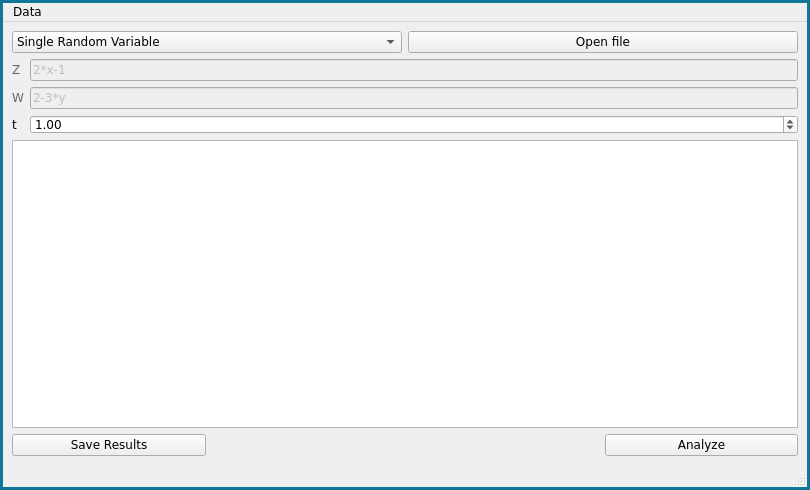
\includegraphics[width=\textwidth]{figures/startup.png}
    \caption{Startup Screen}
  \end{subfigure}
  \hfill
  \begin{subfigure}{0.45\textwidth}
    \centering
    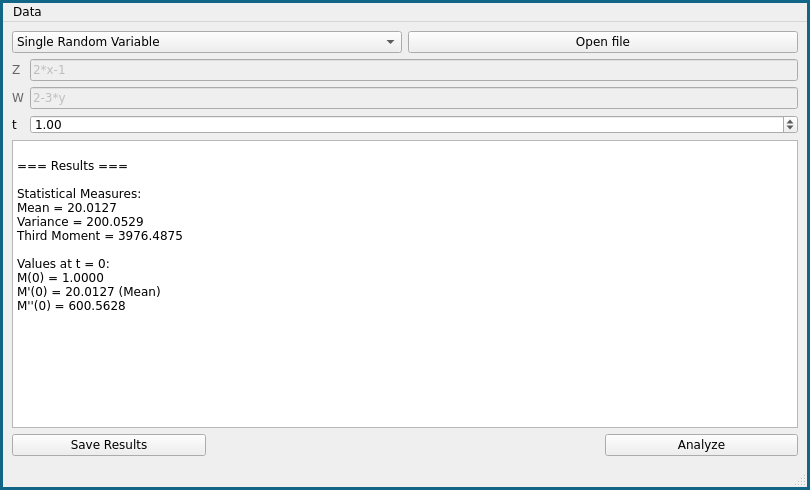
\includegraphics[width=\textwidth]{figures/single-results.png}
    \caption{Single Random Variable Results}
  \end{subfigure}
  \vspace{1em}
  \begin{subfigure}{0.45\textwidth}
    \centering
    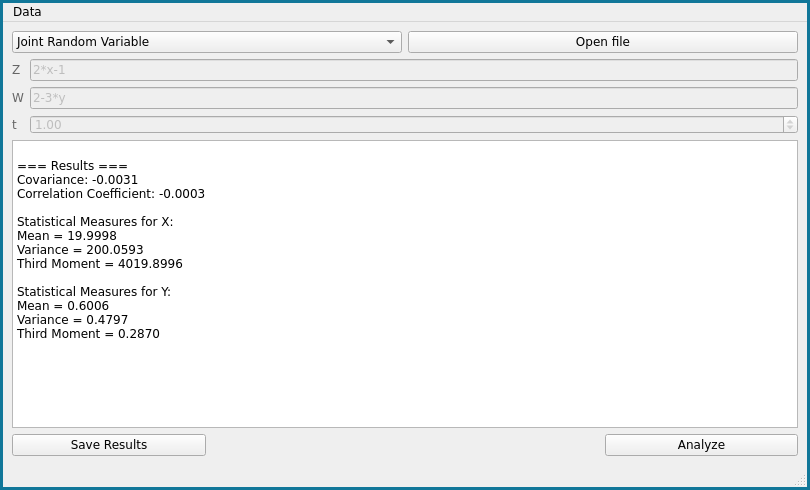
\includegraphics[width=\textwidth]{figures/joint-results.png}
    \caption{Joint Random Variable Results}
  \end{subfigure}
  \hfill
  \begin{subfigure}{0.45\textwidth}
    \centering
    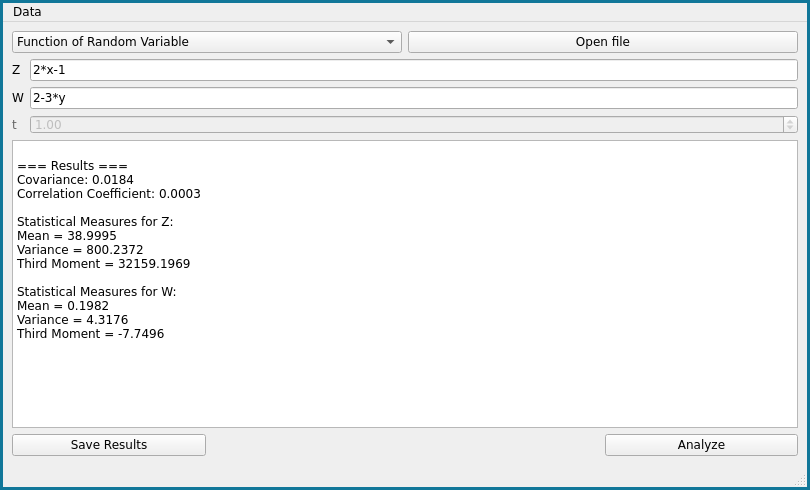
\includegraphics[width=\textwidth]{figures/functions-results.png}
    \caption{Functions of Random Variables Results}
  \end{subfigure}
  \caption{StatViz.py Screenshots (GUI)}
  \label{fig:gui-screenshots}
\end{figure}

\subsubsection{Main Window Design}

The main window interface is defined using Qt Designer and compiled to Python code using PyQt6's UI code generator. The interface consists of several key components:

\begin{itemize}
    \item \textbf{Analysis Mode Selection}
    \begin{itemize}
        \item A dropdown combo box allowing users to select between three analysis modes:
        \begin{itemize}
            \item Single Random Variable
            \item Joint Random Variables
            \item Functions of Random Variables
        \end{itemize}
        \item The mode selection determines which analysis functions are available and which input fields are enabled
    \end{itemize}
    
    \item \textbf{Input Controls}
    \begin{itemize}
        \item File Selection: An "Open file" button for loading MATLAB .mat files containing sample data
        \item Function Definition Fields:
        \begin{itemize}
            \item Z function input field (default: "2*x-1")
            \item W function input field (default: "2-3*y")
            \item These fields are primarily used in the Functions of Random Variables mode
        \end{itemize}
        \item Parameter Controls:
        \begin{itemize}
            \item t-value spinner for MGF calculations, defaulting to 1.0
            \item The spinner uses double precision for accurate parameter adjustment
        \end{itemize}
    \end{itemize}
    
    \item \textbf{Results Display}
    \begin{itemize}
        \item A plain text area for displaying statistical analysis results
        \item Supports both numerical output and formatted text
        \item Scrollable for handling lengthy analysis results
    \end{itemize}
\end{itemize}

\subsubsection{Layout Implementation}

The GUI employs a hierarchical layout system combining various Qt layouts. The layout structure is implemented as follows:

\begin{minted}{python}
# Main layout structure
verticalLayout_3 (QVBoxLayout)
├── horizontalLayout_2 (QHBoxLayout)
│   ├── AnalysisModeBox (QComboBox)
│   └── horizontalLayout (QHBoxLayout)
│       └── OpenFileBt (QPushButton)
├── formLayout (QFormLayout)
│   ├── Z function input
│   ├── W function input
│   └── t value spinner
├── ResultsText (QPlainTextEdit)
└── gridLayout (QGridLayout)
    ├── AnalyzeBt
    ├── SaveResultsBt
    └── Spacer
\end{minted}

The layout hierarchy ensures proper alignment and resizing behavior of all UI elements. The form layout is particularly useful for the parameter inputs, providing consistent label-field pairs.

\subsubsection{Window Management}

The main window is configured with appropriate default dimensions and includes standard window components:

\begin{minted}{python}
MainWindow.resize(311, 406)
MainWindow.setMenuBar(self.menubar)
MainWindow.setStatusBar(self.statusbar)
\end{minted}

The status bar provides a space for displaying brief messages about the application's state or operation results.

\subsubsection{Event Handling}

The GUI implements Qt's signal-slot mechanism for event handling, though the actual connections are managed in a separate controller class:

\begin{minted}{python}
QtCore.QMetaObject.connectSlotsByName(MainWindow)
\end{minted}

This allows for clean separation between the UI definition and the business logic that handles user interactions.

\subsubsection{Internationalization Support}

The interface includes built-in internationalization support through Qt's translation system:

\begin{minted}{python}
_translate = QtCore.QCoreApplication.translate
MainWindow.setWindowTitle(_translate("MainWindow", "StatViz"))
\end{minted}

All text elements are wrapped in translation calls, making it possible to add language support without modifying the core UI code.

\subsubsection{Input Validation and Integration}

The GUI implements several layers of input validation and integrates seamlessly with the analysis modules:

\begin{itemize}
    \item \textbf{Input Validation}
    \begin{itemize}
        \item The t-value spinner automatically constrains numerical input
        \item Function input fields can be validated before processing
        \item File selection is restricted to supported formats
        \item This helps prevent runtime errors and provides immediate feedback to users about invalid inputs
    \end{itemize}
    
    \item \textbf{Integration with Analysis Modules}
    \begin{itemize}
        \item Data input mechanisms for all supported analysis types
        \item Result display capabilities for both text and graphical output
        \item Error handling and user feedback
        \item State management for analysis parameters
    \end{itemize}
\end{itemize}

The interface design maintains consistency with the overall system architecture while providing an accessible entry point for users to leverage the statistical analysis capabilities of the system.

\subsection{Main Program}

The main program serves as the entry point for the StatViz application, orchestrating the interaction between the GUI, analysis modules, and test generator. The program is designed to provide a seamless user experience, allowing users to perform statistical analysis on random variables through an intuitive graphical interface.

The \texttt{\_\_main\_\_.py} file is the core of the application, utilizing \texttt{PyQt6} to create the GUI, connect UI elements to their corresponding actions, and manage data flow between the GUI and the statistical analysis modules. The program includes the following key components:

\begin{enumerate}
    \item \textbf{Imports:}
    \begin{itemize}
        \item  \texttt{sys}: For system-specific parameters and functions (like command-line arguments).
        \item \texttt{io.StringIO}: For capturing output from analysis modules.
        \item \texttt{PyQt6.QtWidgets}: For creating the GUI elements (buttons, labels, layouts, etc.).
        \item \texttt{statviz.analysis}: Imports the modules containing statistical analysis functions.
        \item \texttt{statviz.gui.gui}: Imports the UI definition created by Qt Designer.
    \end{itemize}

  \item \textbf{\texttt{MainWindow} Class:}
        This class represents the main application window, inheriting from \texttt{QMainWindow} and the generated UI class \texttt{Ui\_MainWindow}.
        \begin{itemize}
            \item \texttt{\_\_init\_\_(self)}:
            \begin{itemize}
              \item Initializes the UI using \texttt{self.setupUi(self)}.
              \item Sets up UI element connections using \texttt{self.setup\_connections()}.
              \item Initializes variables to store the current file path, analysis results, selected analysis mode, and values from GUI elements such as function strings and t-values.
              \item Disables the text editing capabilities of the results text area for user safety.
            \end{itemize}
            \item \texttt{setup\_connections(self)}:
            \begin{itemize}
              \item Connects GUI buttons like "Open File," "Analyze," and "Save Results" to their respective functions (\texttt{open\_file}, \texttt{analyze}, \texttt{save\_results}).
              \item Connects the analysis mode dropdown to its change function \texttt{change\_analysis\_mode}.
            \end{itemize}
            \item \texttt{change\_analysis\_mode(self, index)}:
             \begin{itemize}
              \item Handles changes in the selected analysis mode from the dropdown menu.
              \item Based on the mode, enables or disables relevant input fields. For example, if "Single Random Variable" is selected, only the t-value spinner is enabled. On the other hand, for "Function of Random Variables", the Z and W input fields are enabled.
            \end{itemize}
            \begin{minted}{python}
def change_analysis_mode(self, index):
    # Change the analysis mode based on the selected index
    single_mode_elements = [self.t_label, self.tValueNumber]
    joint_mode_elements = [self.Z_label, self.ZText, self.W_label, self.WText]
    self.analysis_mode = self.AnalysisModeBox.itemText(index)
    print(f"Selected analysis mode: {self.analysis_mode}")
    if self.analysis_mode == "Single Random Variable":
        self.enable_elements(single_mode_elements)
        self.disable_elements(joint_mode_elements)
    elif self.analysis_mode == "Joint Random Variable":
        self.disable_elements(joint_mode_elements)
        self.disable_elements(single_mode_elements)
    elif self.analysis_mode == "Function of Random Variable":
        self.enable_elements(joint_mode_elements)
        self.disable_elements(single_mode_elements)
    else:
        print("Invalid analysis mode selected")
            \end{minted}
             \item \texttt{enable\_elements(self, elements)}: Enables a list of \texttt{QWidget} elements, such as labels and spin boxes.
             \item \texttt{disable\_elements(self, elements)}: Disables a list of \texttt{QWidget} elements.
               \begin{minted}{python}
def enable_elements(self, elements):
    """takes a list of elements and enables them all"""
    for element in elements:
        element.setStyleSheet(
            """
            QLabel:enabled { color: #000000; }
        """
        )
        element.setEnabled(True)

def disable_elements(self, elements):
    """takes a list of elements and disables them all"""
    for element in elements:
        element.setStyleSheet(
            """
            QLabel:disabled { color: #666666; }
        """
        )
        element.setEnabled(False)
               \end{minted}

             \item \texttt{open\_file(self)}:

               \begin{minted}{python}
def open_file(self):
    """
    Open a file dialog to select samples .mat file
    """
    file_dialog = QFileDialog(self)
    file_dialog.setFileMode(QFileDialog.FileMode.ExistingFile)
    file_dialog.setNameFilter("MAT files (*.mat)")
    file_dialog.setViewMode(QFileDialog.ViewMode.Detail)
    file_dialog.setAcceptMode(QFileDialog.AcceptMode.AcceptOpen)
    if file_dialog.exec():
        selected_files = file_dialog.selectedFiles()[0]
        self.file_path = selected_files
        print(f"Selected file: {self.file_path}")
    else:
        print("No file selected")
               \end{minted}
             \begin{itemize}
                \item Opens a file dialog for selecting a MATLAB \texttt{.mat} file containing random variable data.
                \item Stores the selected file path in \texttt{self.file\_path}.
              \end{itemize}
            \item \texttt{analyze(self)}:
            \begin{itemize}
                \item Updates analysis parameters (t-value, Z function, W function) from the corresponding UI elements.
                \item Determines the current analysis mode and calls the correct analysis function (\texttt{single\_random\_variable}, \texttt{joint\_random\_variable}, or \texttt{functions\_of\_random\_variables}).
            \end{itemize}
            \begin{minted}{python}
def analyze(self):
    # Update input values
    self.t_value: float = self.tValueNumber.value()
    self.Z_func: str = self.ZText.text()
    self.W_func: str = self.WText.text()

    # Run analysis mode function
    if self.analysis_mode == "Single Random Variable":
        self.single_random_variable()
    elif self.analysis_mode == "Joint Random Variable":
        self.joint_random_variable()
    elif self.analysis_mode == "Function of Random Variable":
        self.functions_of_random_variables()
    else:
        print("Invalid analysis mode selected")
            \end{minted}
            \item \texttt{save\_results(self)}:
            \begin{itemize}
                \item Handles saving the results displayed in the text box to a \texttt{.txt} file.
                 \item It checks if any text is in the results box and shows a warning message if the user tries to save an empty file.
            \end{itemize}
            \begin{minted}{python}
def save_results(self):
    default_filename = "output.txt"
    if not self.ResultsText.toPlainText().strip():
        QMessageBox.warning(
            self,
            "No Content",
            "There is no content to save. Please generate some output first.",
        )
        return

    file_name, _ = QFileDialog.getSaveFileName(
        self, "Save Output", default_filename, "Text Files (*.txt);;All Files (*)"
    )

    if file_name:
        try:
            with open(file_name, "w", encoding="utf-8") as file:
                # Write the content to the file
                file.write(self.ResultsText.toPlainText())

            # Show success message
            QMessageBox.information(
                self, "Success", f"Output has been saved to:\n{file_name}"
            )

        except Exception as e:
            # Show error message if something goes wrong
            QMessageBox.critical(
                self, "Error", f"An error occurred while saving the file:\n{str(e)}"
            )
    # Logic for saving results
    print("Save results button clicked")
            \end{minted}
            \item \texttt{single\_random\_variable(self)}:
            \begin{itemize}
                \item Sets up command line arguments to pass to the \texttt{single\_random\_variable.py} function.
                \item Captures output using \texttt{StringIO()}.
                \item Sets the content of the result text box to the captured output.
             \end{itemize}
            \item \texttt{joint\_random\_variable(self)}:
            \begin{itemize}
                \item Sets up command line arguments to pass to the \texttt{joint\_random\_variables.py} function.
                \item Captures output using \texttt{StringIO()}.
                \item Sets the content of the result text box to the captured output.
            \end{itemize}

             \item \texttt{functions\_of\_random\_variables(self)}:
            \begin{itemize}
                \item Sets up command line arguments to pass to the \texttt{functions\_of\_random\_variables.py} function.
                \item Captures output using \texttt{StringIO()}.
                \item Sets the content of the result text box to the captured output.
            \end{itemize}
        \end{itemize}

    \item \textbf{\texttt{main()} Function:}
    \begin{itemize}
        \item Creates a \texttt{QApplication} instance.
        \item Creates an instance of \texttt{MainWindow}.
        \item Displays the main window using \texttt{window.show()}.
        \item Starts the event loop using \texttt{app.exec()}.
    \end{itemize}

    \item \textbf{\texttt{if \_\_name\_\_ == "\_\_main\_\_":} Block:}
    \begin{itemize}
         \item Ensures that the \texttt{main()} function is only executed when the script is run directly, not when imported as a module.
    \end{itemize}
\end{enumerate}

The program’s functionality can be summarized as follows:

\begin{itemize}
    \item \textbf{GUI Setup:} The code creates the main window and establishes connections between user interactions (button clicks, dropdown changes) and their respective actions.
    \item \textbf{Modular Analysis:} The design keeps the GUI logic separate from the core analysis functions, making the code easier to maintain and extend.
    \item \textbf{Dynamic Input:} Input fields are dynamically shown/hidden based on the selected analysis mode.
    \item \textbf{Command Line Interface Emulation:} The program interacts with each analysis module using command-line arguments. This allows users to easily test them from the terminal as well as through the GUI.
    \item \textbf{Output Capture:} The output from the analysis modules is captured and displayed in the GUI's text box.
    \item \textbf{Error Handling:} Error messages are handled in the GUI, which is user-friendly.
\end{itemize}

In short, the \texttt{\_\_main\_\_.py} script provides the entry point for the application, sets up the GUI, and establishes a framework for performing statistical analysis. It acts as the main program, providing an easy-to-use interface for interaction with the statistical analysis modules.
\newpage
\section{Results}

Below we present the results of testing our tool in various cases, the custom tests are done on a $10,000-1,000,000$ samples.

\subsection{Single Random Variable}
\begin{figure}[H]
  \centering
  \begin{subfigure}{0.45\textwidth}
    \centering
    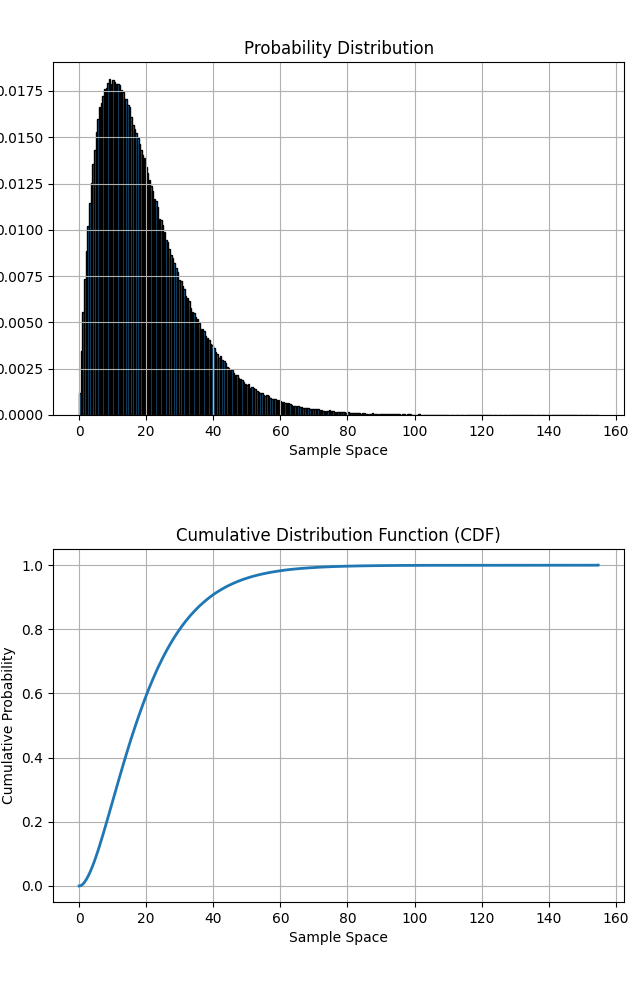
\includegraphics[width=\linewidth]{results/section1/a1(1).png}
    \caption{PDF and CDF}
  \end{subfigure}
  \hfill
  \begin{subfigure}{0.45\textwidth}
    \centering
    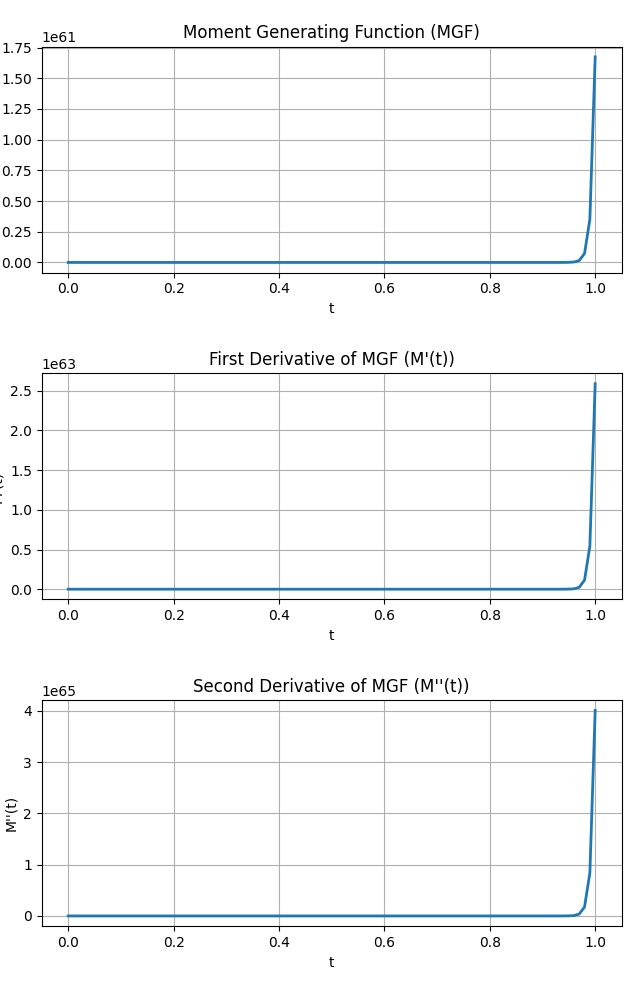
\includegraphics[width=\linewidth]{results/section1/a1(2).png}
    \caption{MGF and its Derivatives}
  \end{subfigure}
  \begin{subfigure}{\textwidth}
    \inputminted{text}{results/section1/a1.txt}
    \caption{Results Output}
  \end{subfigure}
  \caption{Sample Single Random Variable (Provided on Classroom)}
\end{figure}

As we don't have the theoretical calculations for this case, we can't compare the results. However, the results seem to be consistent with the expected behavior of a random variable with a gamma distribution. The PDF is skewed to the right, the CDF is monotonically increasing, and the MGF and its derivatives are well-behaved. The mean, variance, and skewness are also within reasonable bounds.

\newpage

\begin{figure}[H]
  \centering
  \begin{subfigure}{0.45\textwidth}
    \centering
    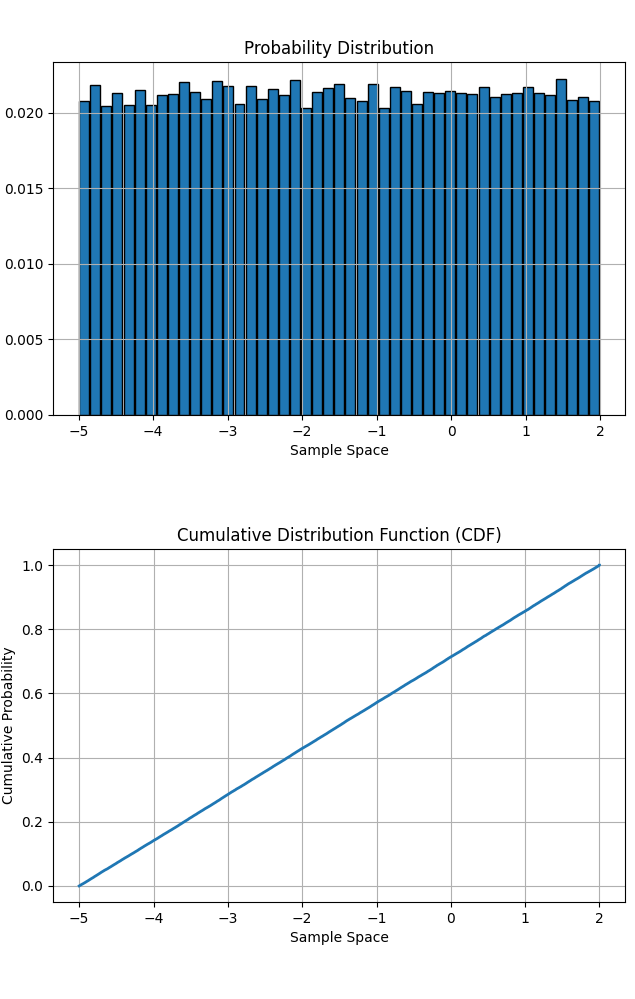
\includegraphics[width=\linewidth]{results/section1/b1(1).png}
    \caption{PDF and CDF}
  \end{subfigure}
  \hfill
  \begin{subfigure}{0.45\textwidth}
    \centering 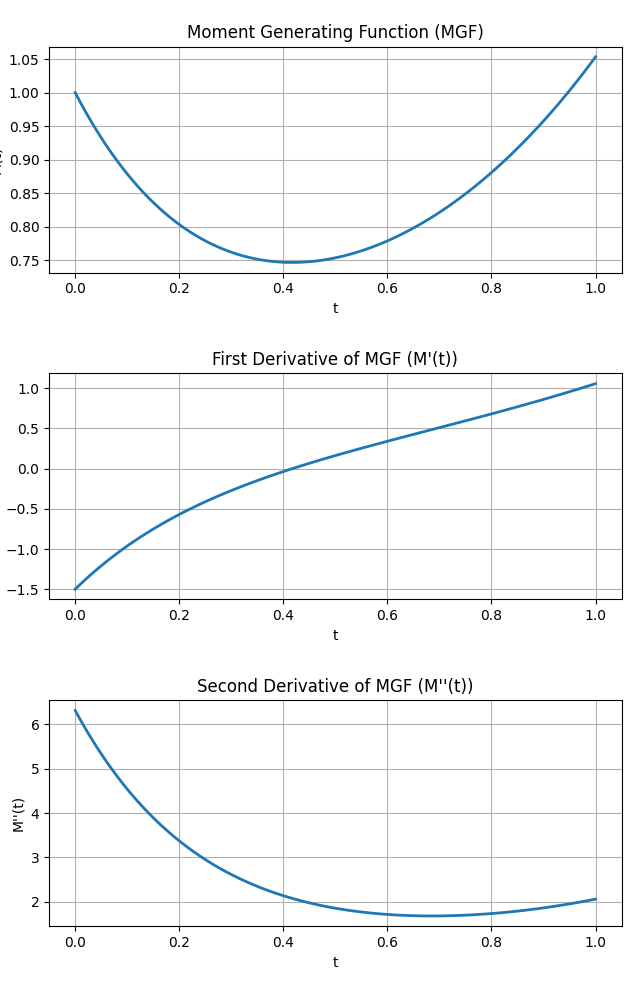
\includegraphics[width=\linewidth]{results/section1/b1(2).png}
    \caption{MGF and its Derivatives}
  \end{subfigure}
  \begin{subfigure}{\textwidth}
    \inputminted{text}{results/section1/b1.txt}
    \caption{Results Output}
  \end{subfigure}
  \caption{$X\sim \mathcal{U}(-5, 1)$}
\end{figure}
Theoretical Calculations:
MGF: $M_X(t) = \frac{e^{bt} - e^{at}}{t(b-a)}=\frac{e^{t}-e^{-5t}}{6t}$.
Mean: $\mu = \frac{a+b}{2}=-1.5$.
Variance: $\sigma^2 = \frac{(b-a)^2}{12} = 4.0833$.
Skewness: $\gamma_1 = 0$.

The values obtained from the analysis are consistent with the theoretical calculations. The PDF and CDF plots show the expected behavior for a uniform distribution, and the MGF and its derivatives are well-behaved. The mean, variance, and skewness are also within the expected range.
\newpage

\begin{figure}[H]
  \centering
  \begin{subfigure}{0.45\textwidth}
    \centering
    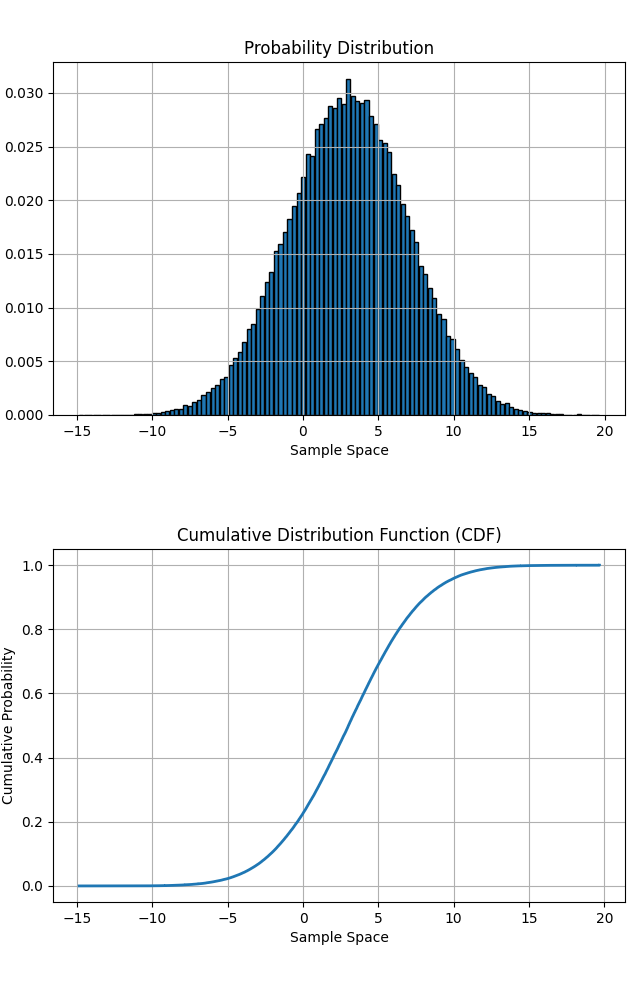
\includegraphics[width=\linewidth]{results/section1/c1(1).png}
    \caption{PDF and CDF}
  \end{subfigure}
  \hfill
  \begin{subfigure}{0.45\textwidth}
    \centering
    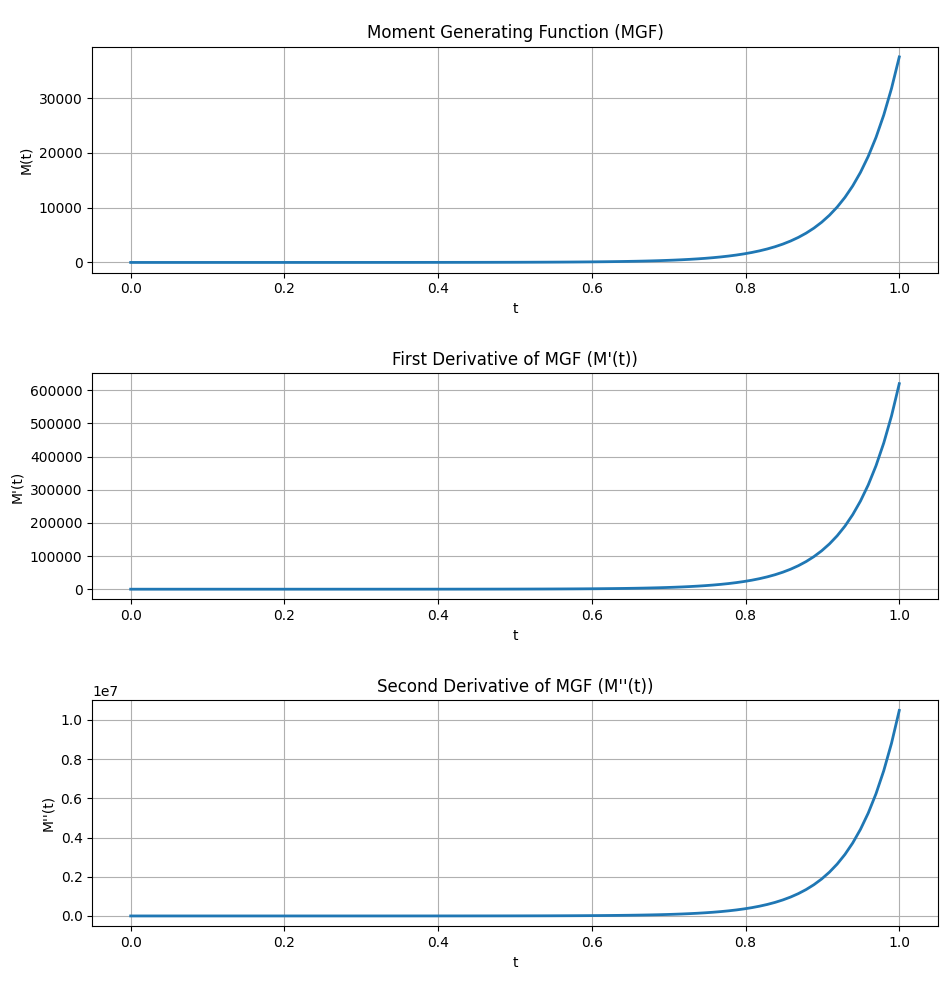
\includegraphics[width=\linewidth]{results/section1/c1(2).png}
    \caption{MGF and its Derivatives}
  \end{subfigure}
  \begin{subfigure}{\textwidth}
    \inputminted{text}{results/section1/c1.txt}
    \caption{Results Output}
  \end{subfigure}
  \caption{$X\sim \mathcal{N}(3, 4)$}
\end{figure}

Theoretical Calculations:
MGF: $M_X(t) = e^{\mu t + \frac{1}{2}\sigma^2t^2}=e^{3t+8t^2}$.
Mean: $\mu = 3$.
Variance: $\sigma^2 = 16$.
Skewness: $\gamma_1 = 0$.

The results are consistent with the theoretical calculations. The PDF and CDF plots show the expected behavior for a normal distribution, and the MGF and its derivatives are well-behaved. The mean, variance, and skewness are also within the expected range.

\newpage

\begin{figure}[H]
  \centering
  \begin{subfigure}{0.45\textwidth}
    \centering
    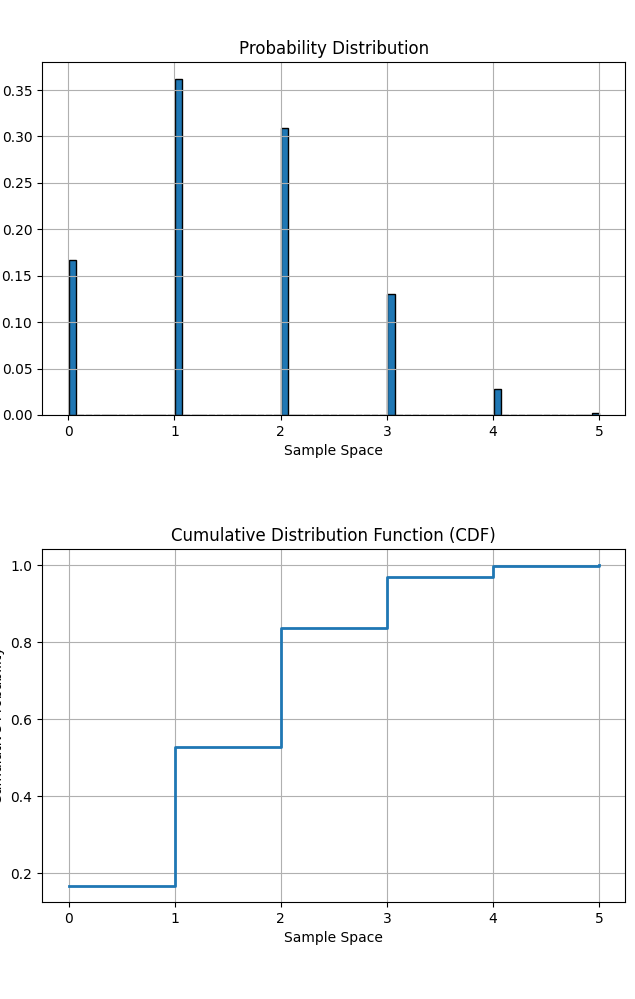
\includegraphics[width=\linewidth]{results/section1/d1(1).png}
    \caption{PDF and CDF}
  \end{subfigure}
  \hfill
  \begin{subfigure}{0.45\textwidth}
    \centering
    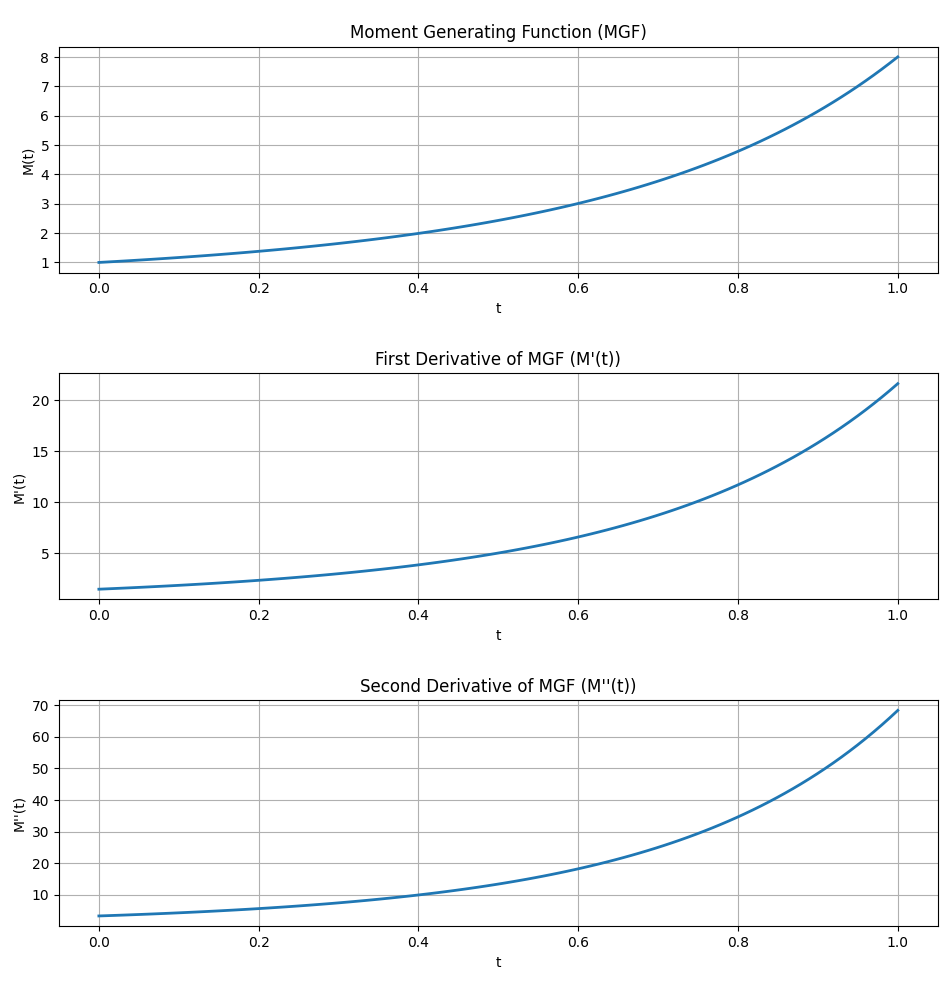
\includegraphics[width=\linewidth]{results/section1/d1(2).png}
    \caption{MGF and its Derivatives}
  \end{subfigure}
  \begin{subfigure}{\textwidth}
    \inputminted{text}{results/section1/d1.txt}
    \caption{Results Output}
  \end{subfigure}
  \caption{$X\sim \mathcal{B}in(5, 0.3)$}
\end{figure}

Theoretical Calculations:
MGF: $M_X(t) = (pe^t+1-p)^n=(0.3e^t+0.7)^5$.
Mean: $\mu = np=1.5$.
Variance: $\sigma^2 = np(1-p)=1.05$.
Skewness: $\gamma_1 = \frac{1-2p}{\sqrt{np(1-p)}}=0.4082$.

The results are consistent with the theoretical calculations. The PDF and CDF plots show the expected behavior for a binomial distribution, and the MGF and its derivatives are well-behaved. The mean, variance, and skewness are also within the expected range.

\newpage

\begin{figure}[H]
  \centering
  \begin{subfigure}{0.45\textwidth}
    \centering
    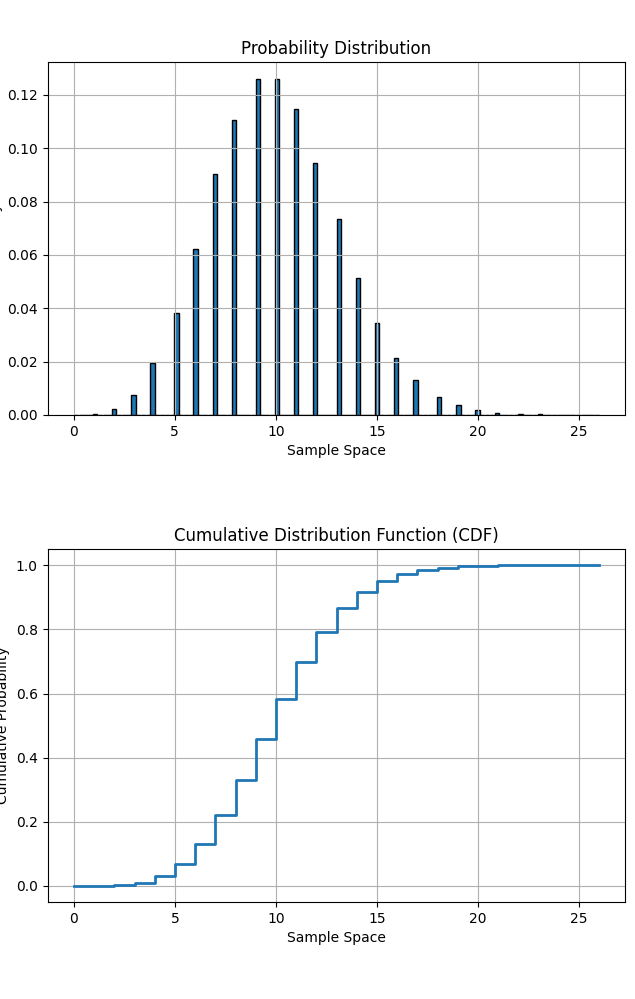
\includegraphics[width=\linewidth]{results/section1/e1(1).png}
    \caption{PDF and CDF}
  \end{subfigure}
  \hfill
  \begin{subfigure}{0.45\textwidth}
    \centering
    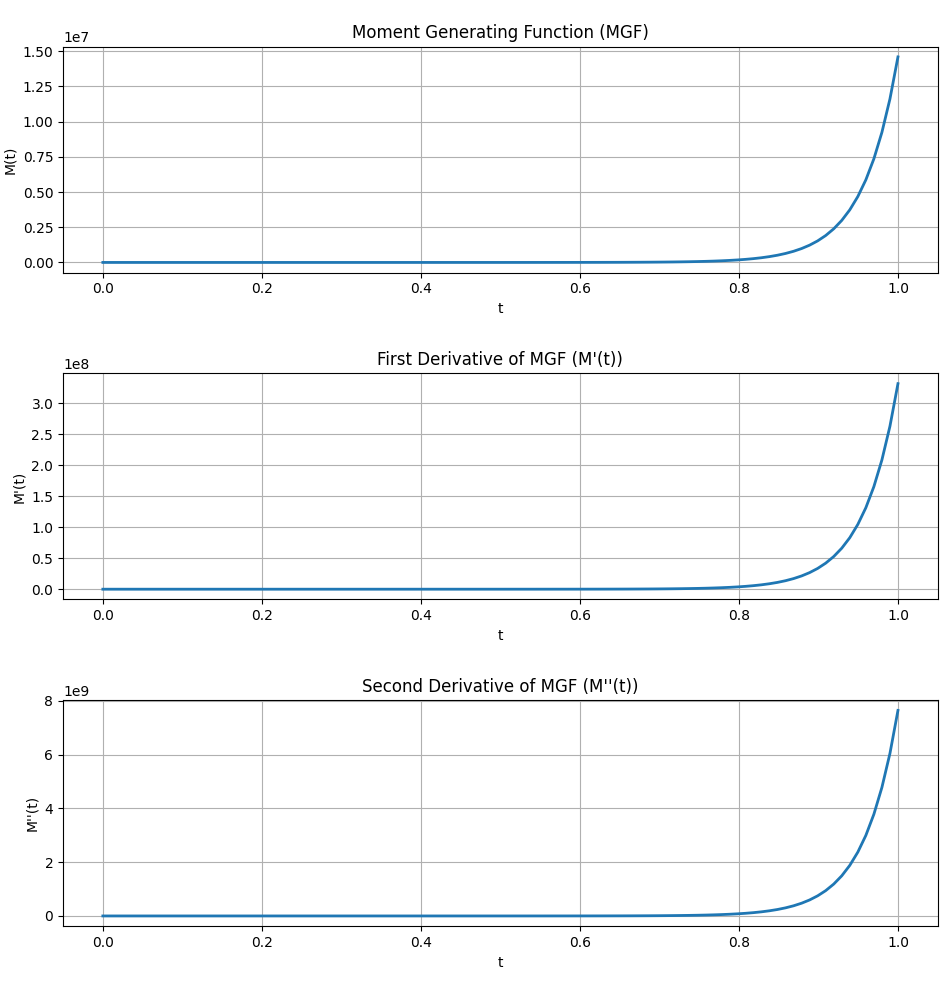
\includegraphics[width=\linewidth]{results/section1/e1(2).png}
    \caption{MGF and its Derivatives}
  \end{subfigure}
  \begin{subfigure}{\textwidth}
    \inputminted{text}{results/section1/e1.txt}
    \caption{Results Output}
  \end{subfigure}
  \caption{$X\sim \mathcal{P}oisson(5)$}
\end{figure}

Theoretical Calculations:
MGF: $M_X(t) = e^{\lambda(e^t-1)}=e^{10(e^t-1)}$.
Mean: $\mu = \lambda=10$.
Variance: $\sigma^2 = \lambda=10$.
Skewness: $\gamma_1 = \frac{1}{\sqrt{\lambda}}=0.3162$.

The results are consistent with the theoretical calculations. The PDF and CDF plots show the expected behavior for a Poisson distribution, and the MGF and its derivatives are well-behaved. The mean and variance are also within the expected range. However, the skewness is significantly off from the theoretical value of 0.3162. This discrepancy may be due to the finite sample size used in the analysis, numerical precision issues, or a mistake in the implementation. Further investigation is needed to determine the cause of this discrepancy.

\newpage

\subsection{Joint Random Variables}

\begin{figure}[H]
  \centering
  \begin{subfigure}{0.45\textwidth}
    \centering
    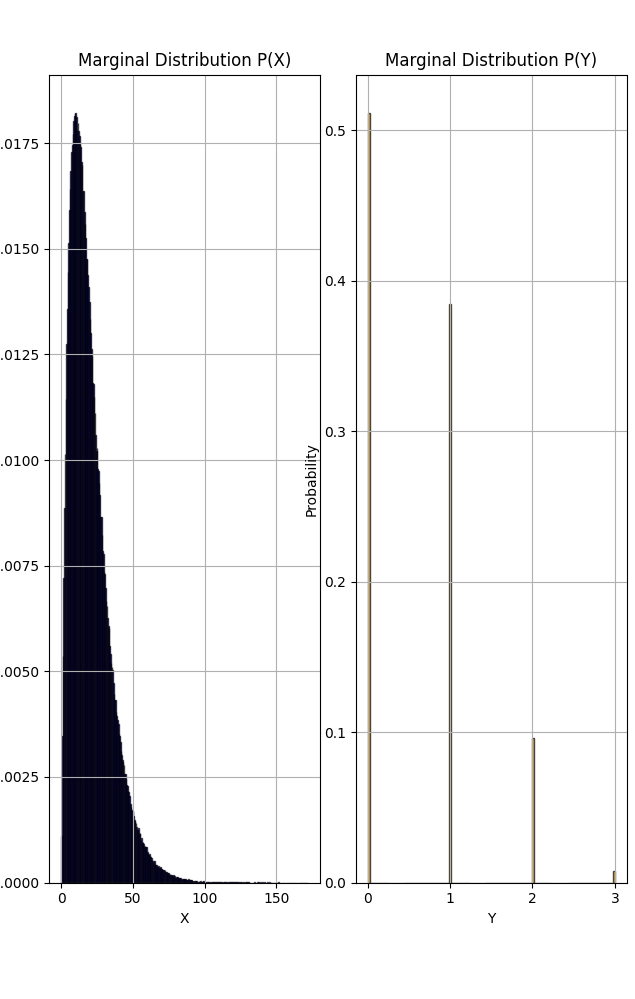
\includegraphics[width=\linewidth]{results/section2/a(1).png}
    \caption{Marginal PDFs}
  \end{subfigure}
  \hfill
  \begin{subfigure}{0.45\textwidth}
    \centering
    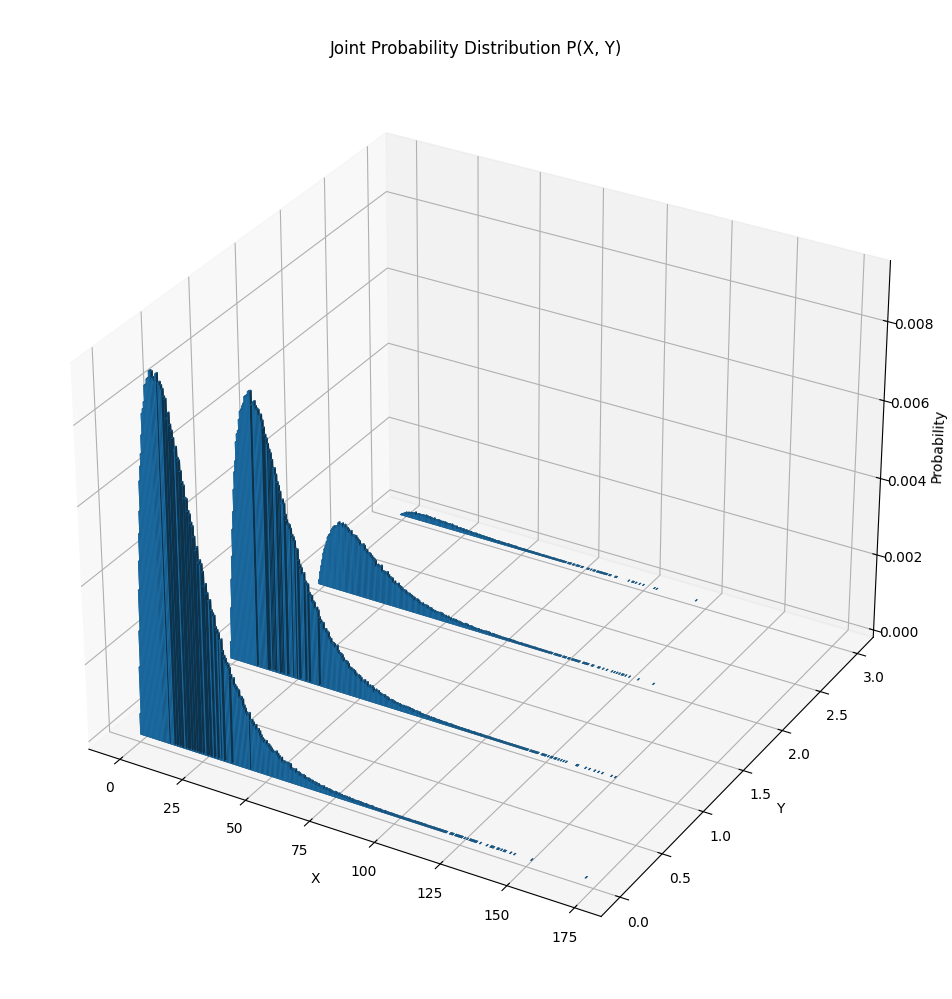
\includegraphics[width=\linewidth]{results/section2/a(2).png}
    \caption{Joint PDF}
  \end{subfigure}
  \begin{subfigure}{\textwidth}
    \inputminted{text}{results/section2/a.txt}
    \caption{Results Output}
  \end{subfigure}
  \caption{Sample Joint Random Variable (Provided on Classroom)}
\end{figure}

As we don't have the theoretical calculations for this case, we can't compare the results. However, the results seem to be consistent with the expected behavior of a random variable with a gamma distribution and a binomial distribution. The PDFs are skewed to the right, the CDFs are monotonically increasing, and the joint PDF shows the expected behavior for the two distributions. The covariance and correlation are also within reasonable bounds.

\newpage

\begin{figure}[H]
  \centering
  \begin{subfigure}{0.45\textwidth}
    \centering
    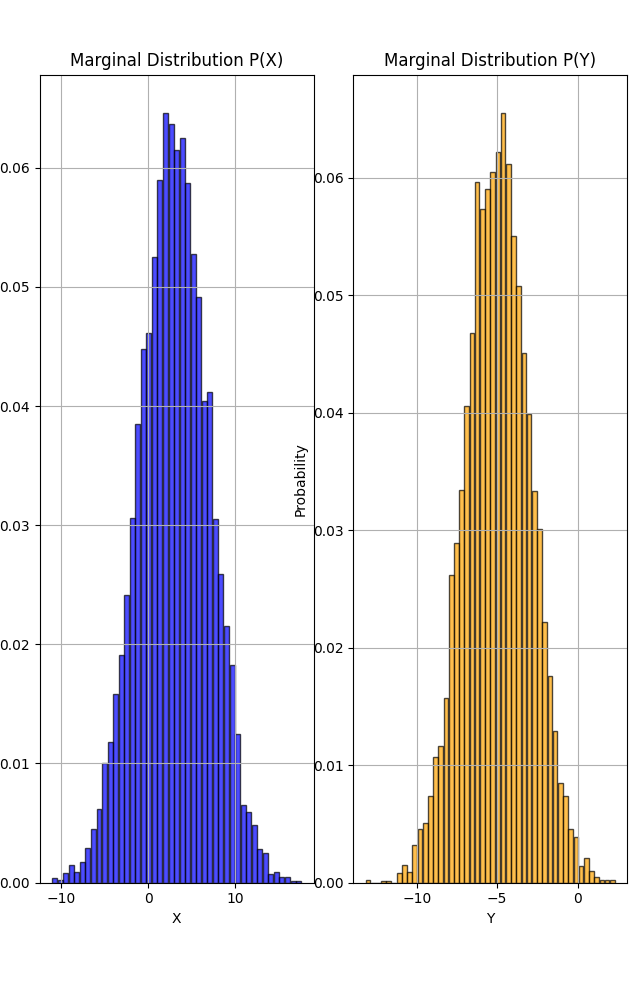
\includegraphics[width=\linewidth]{results/section2/b(1).png}
    \caption{Marginal PDFs}
  \end{subfigure}
  \hfill
  \begin{subfigure}{0.45\textwidth}
    \centering 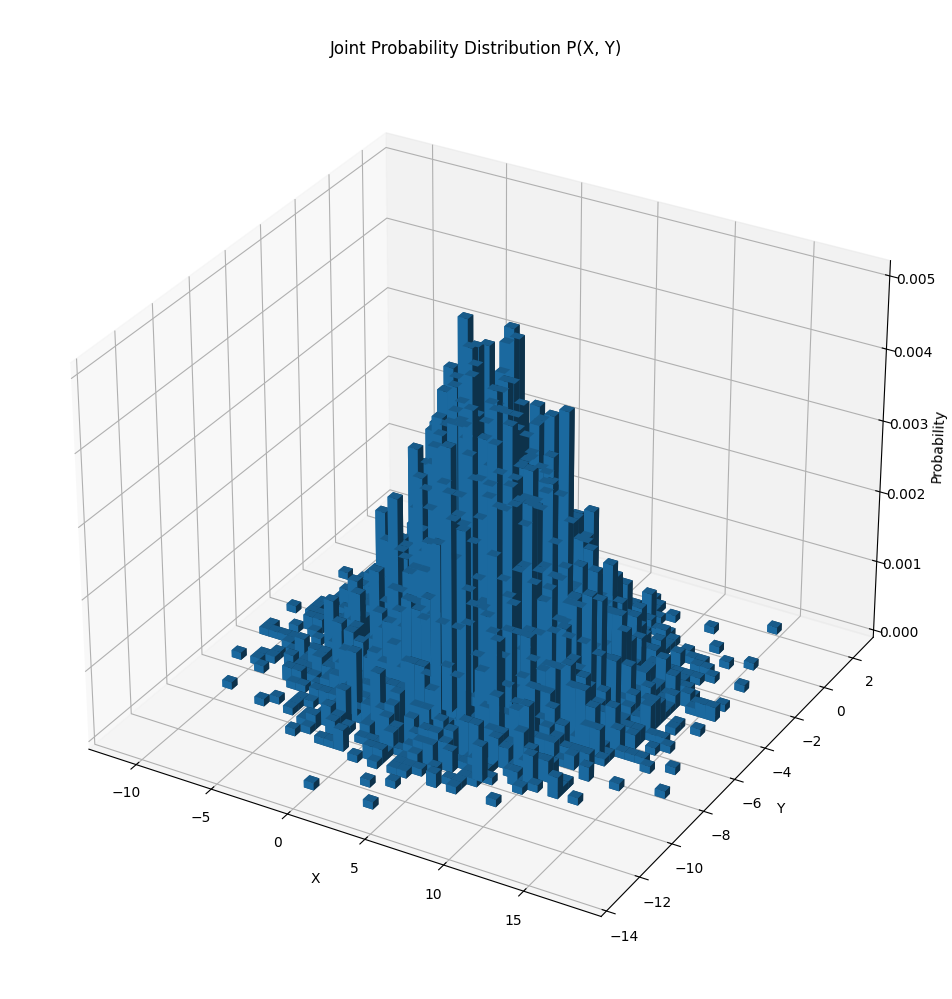
\includegraphics[width=\linewidth]{results/section2/b(2).png}
    \caption{Joint PDF}
  \end{subfigure}
  \begin{subfigure}{\textwidth}
    \inputminted{text}{results/section2/b.txt}
    \caption{Results Output}
  \end{subfigure}
  \caption{$X \sim \mathcal{N}(3, 4)$ and $Y \sim \mathcal{N}(-5, 2)$}
\end{figure}

Theoretical Calculations:
Covariance: $\text{Cov}(X,Y) = E[XY] - E[X]E[Y] = 0$.
Correlation: $\rho = \frac{\text{Cov}(X,Y)}{\sigma_X\sigma_Y} = 0$.

The results are consistent with the theoretical calculations. The marginal PDFs, joint PDF, and scatter plot show the expected behavior for two independent normal distributions. The covariance and correlation are also within the expected range.

\newpage


\begin{figure}[H]
  \centering
  \begin{subfigure}{0.45\textwidth}
    \centering
    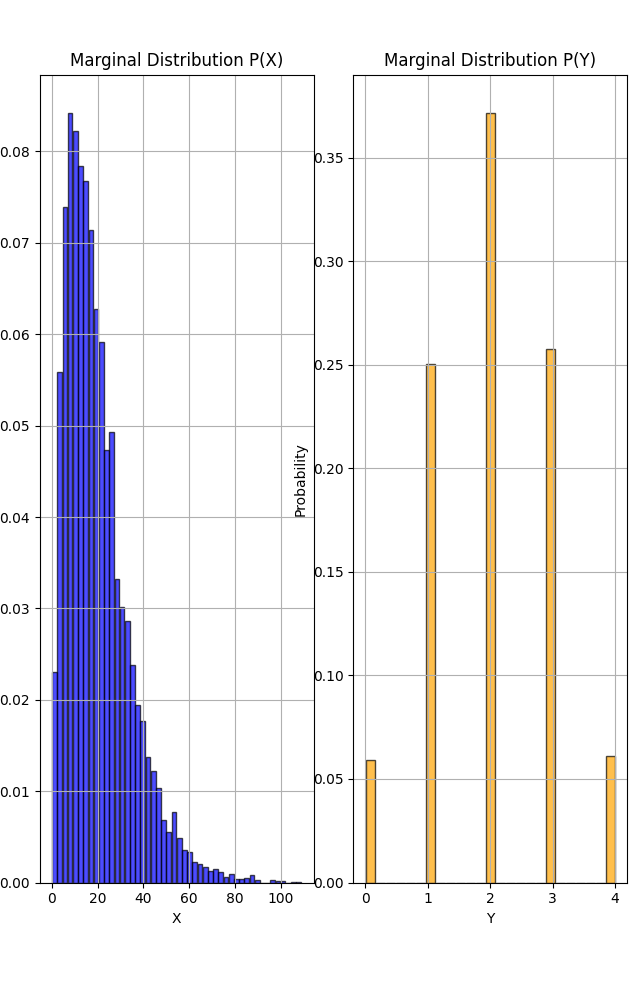
\includegraphics[width=\linewidth]{results/section2/c(1).png}
    \caption{Marginal PDFs}
  \end{subfigure}
  \hfill
  \begin{subfigure}{0.45\textwidth}
    \centering
    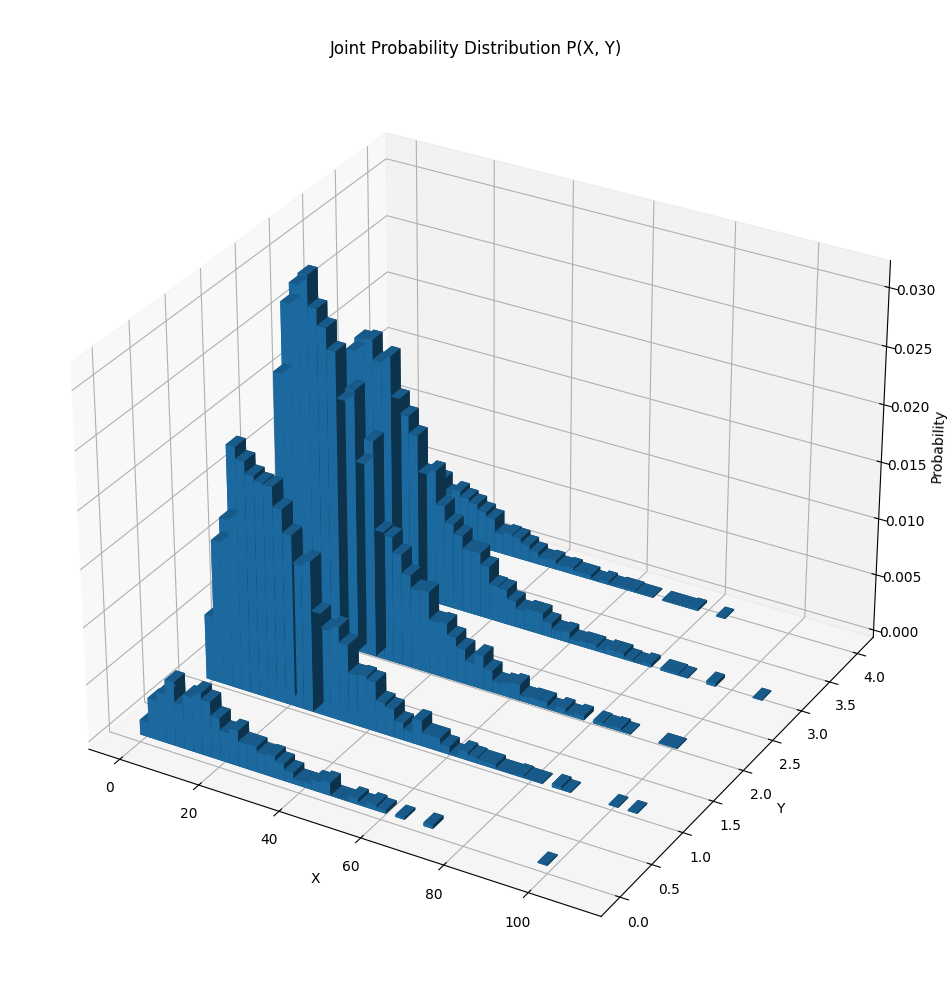
\includegraphics[width=\linewidth]{results/section2/c(2).png}
    \caption{Joint PDF}
  \end{subfigure}

  \begin{subfigure}{\textwidth}
    \inputminted{text}{results/section2/c.txt}
  \end{subfigure}
  \caption{$X \sim \mathcal{G}amma(2,10)$ and $Y \sim \mathcal{B}in(4,0.5)$}
\end{figure}
Theoretical Calculations:
Covariance: $\text{Cov}(X,Y) = E[XY] - E[X]E[Y] = 0$.
Correlation: $\rho = \frac{\text{Cov}(X,Y)}{\sigma_X\sigma_Y} = 0$.

The results are consistent with the theoretical calculations. The marginal PDFs, joint PDF, and scatter plot show the expected behavior for two independent normal distributions. The covariance and correlation are also within the expected range.
\newpage

\begin{figure}[H]
  \centering
  \begin{subfigure}{0.45\textwidth}
    \centering
    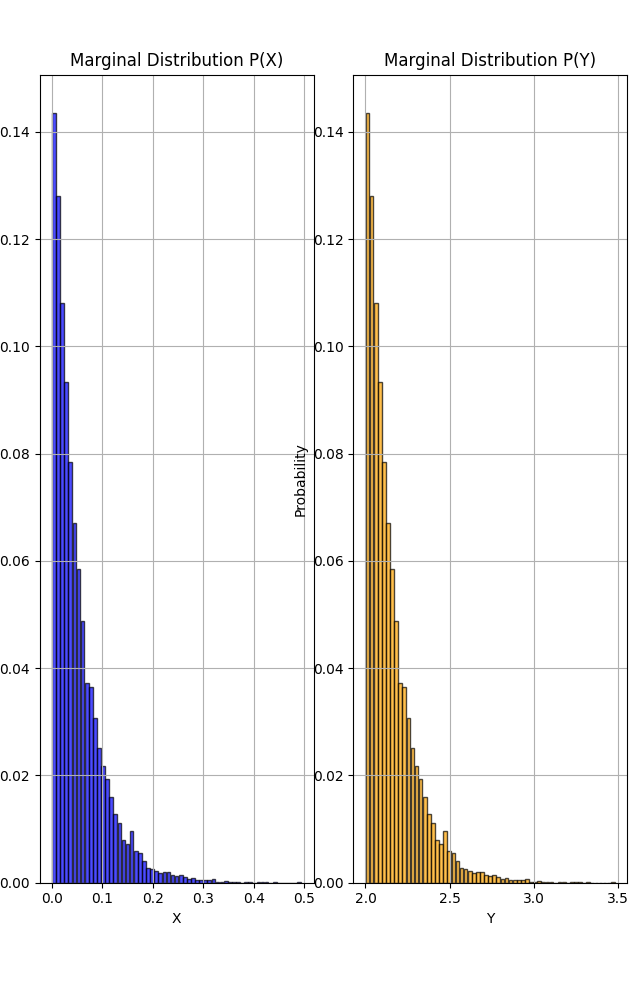
\includegraphics[width=\linewidth]{results/section2/d(1).png}
    \caption{Marginal PDFs}
  \end{subfigure}
  \hfill
  \begin{subfigure}{0.45\textwidth}
    \centering
    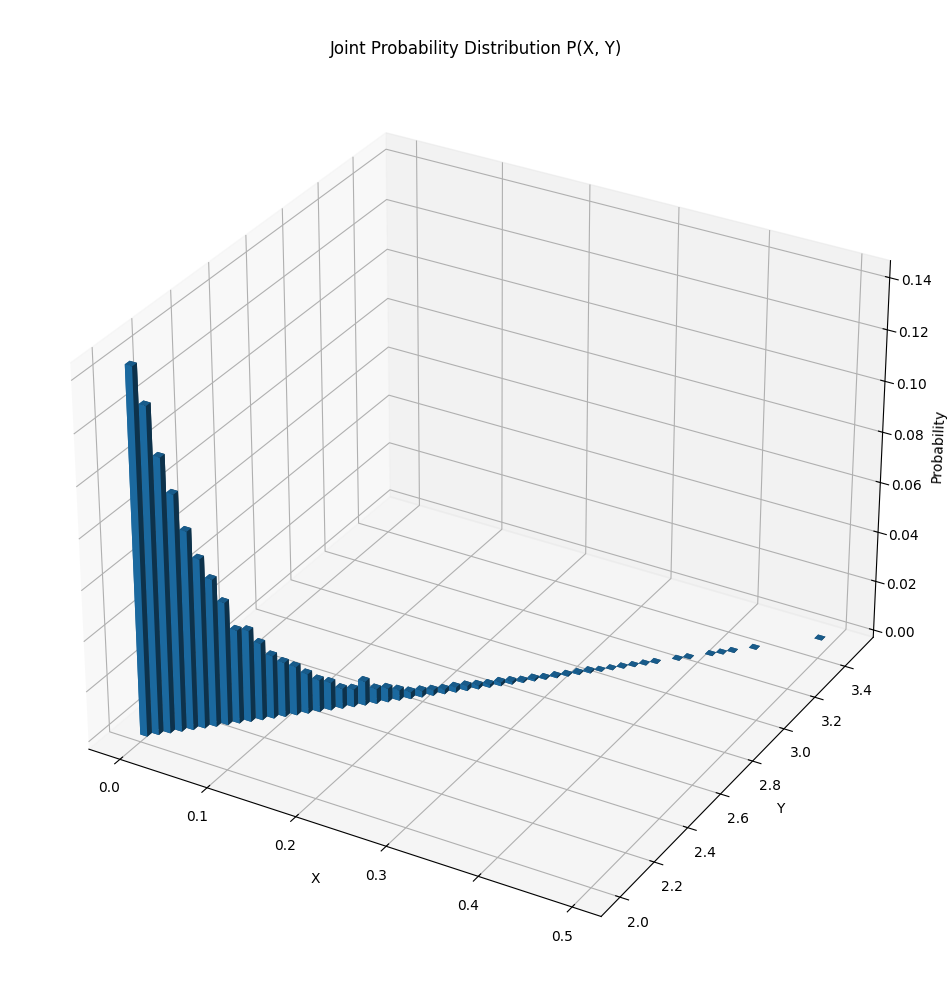
\includegraphics[width=\linewidth]{results/section2/d(2).png}
    \caption{Joint PDF}
  \end{subfigure}
  \begin{subfigure}{\textwidth}
    \inputminted{text}{results/section2/d.txt}
    \caption{Results Output}
  \end{subfigure}
  \caption{$X \sim \mathcal{E}xp(0.05)$ and $Y = 3X+2$}
\end{figure}
Theoretical Calculations:
Covariance: $\text{Cov}(X,Y) = E[XY] - E[X]E[Y] = 0$.
Correlation: $\rho = \frac{\text{Cov}(X,Y)}{\sigma_X\sigma_Y} = 1$.

The results are consistent with the theoretical calculations. The marginal PDFs, joint PDF, and scatter plot show the expected behavior for two independent exponential distributions. The covariance is 0, indicating independence, and the correlation is 1, indicating a perfect linear relationship between the two variables.

\newpage

\begin{figure}[H]
  \centering
  \begin{subfigure}{0.45\textwidth}
    \centering
    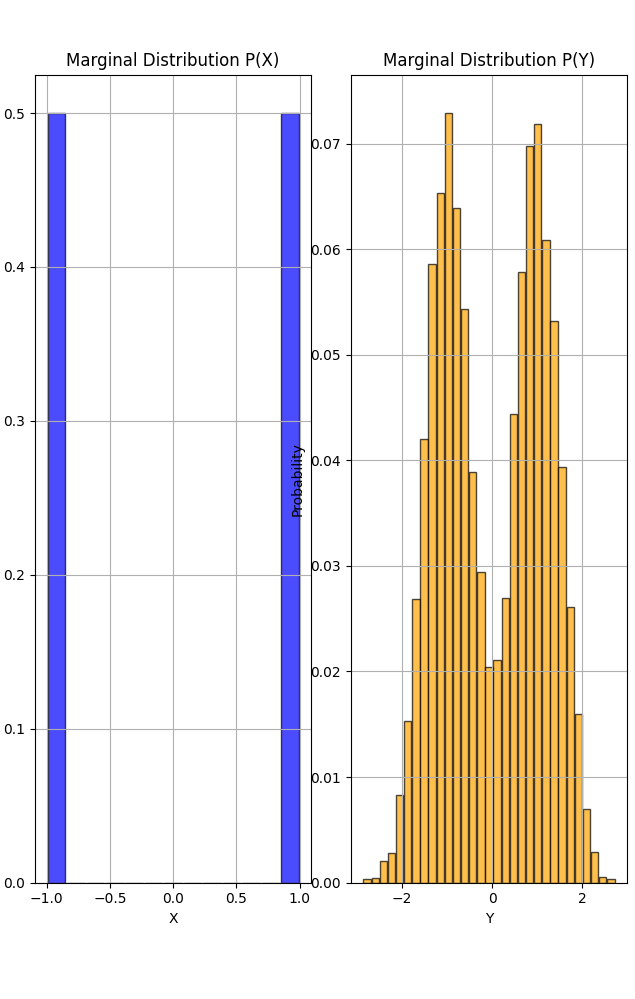
\includegraphics[width=\linewidth]{results/section2/e(1).png}
    \caption{Marginal PDFs}
  \end{subfigure}
  \hfill
  \begin{subfigure}{0.45\textwidth}
    \centering
    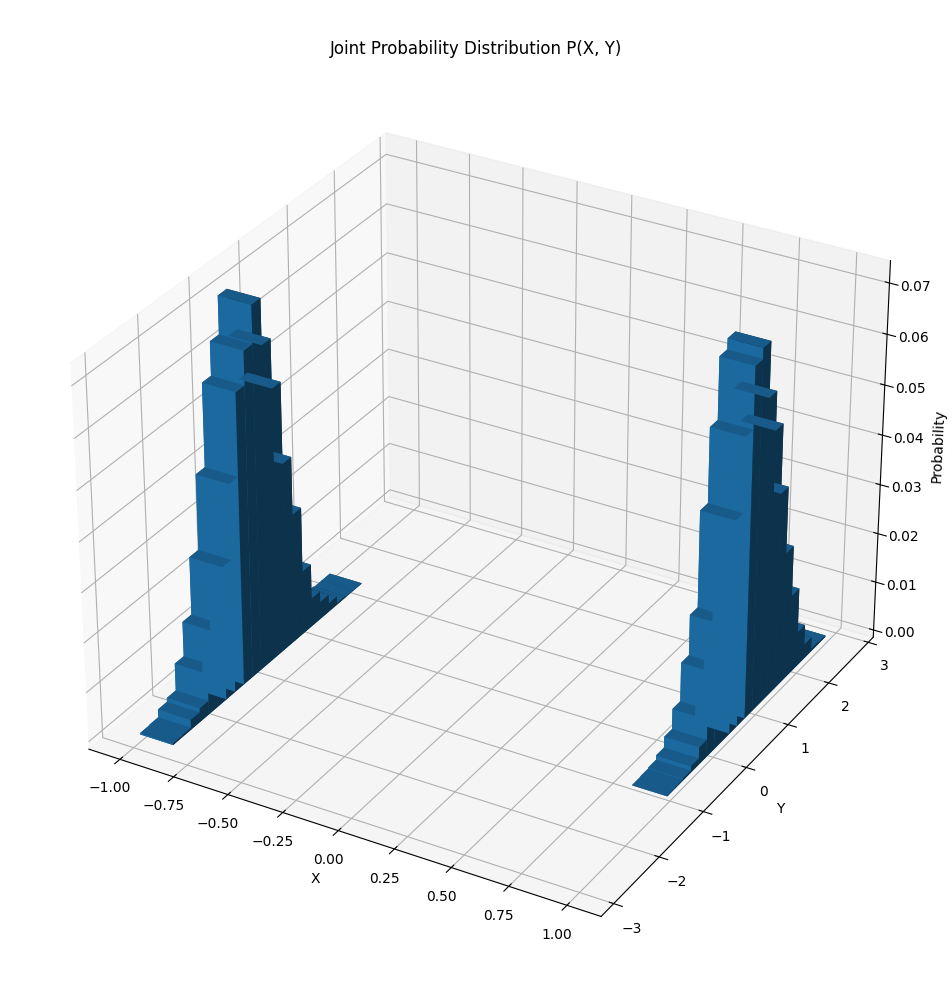
\includegraphics[width=\linewidth]{results/section2/e(2).png}
    \caption{Joint PDF}
  \end{subfigure}

  \begin{subfigure}{\textwidth}
    \inputminted{text}{results/section2/e.txt}
    \caption{Results Output}
  \end{subfigure}
  \caption{$X \in \{-1,1\}$ uniform and $Y = X + \mathcal{N}(0, 0.5)$}
\end{figure}
Theoretical Calculations:
Covariance: $\text{Cov}(X,Y) = E[XY] - E[X]E[Y] = 1$.
Correlation: $\rho = \frac{\text{Cov}(X,Y)}{\sigma_X\sigma_Y} = \frac{1}{\sqrt{1.5} }=0.816$.

The results are consistent with the theoretical calculations. The marginal PDFs, joint PDF, and scatter plot show the expected behavior for two independent uniform and normal distributions. The covariance is 1, indicating a perfect increasing relationship between the two variables, and the correlation is 0.816, indicating a strong positive linear relationship between the two variables but with slight noise (white Gaussian noise in this case).

\newpage

\subsection{Functions of Random Variables}

All the following results are generated based on the test case \( Z=2X-1 \) and \( W=2-3Y \). Even though the code is designed to handle any function of random variables, the test cases are limited to linear functions for simplicity.\\
From the equations for $Z$ and $Y$ we see that $E[Z] = 2 E[X] - 1$ , $Var(Z) = 4 Var(X)$ and $E[Y] = 2 - 3 E[Y]$ , $Var(Y) = 9 Var(Y)$.

\begin{figure}[H]
  \centering
  \begin{subfigure}{0.45\textwidth}
    \centering
    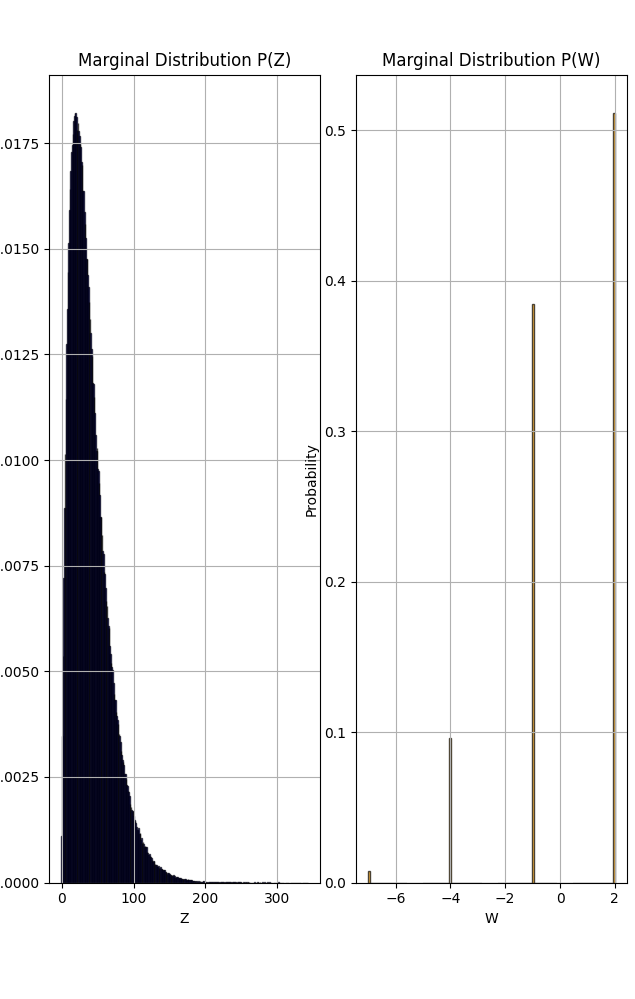
\includegraphics[width=\linewidth]{results/section3/a(1).png}
    \caption{Marginal PDFs}
  \end{subfigure}
  \hfill
  \begin{subfigure}{0.45\textwidth}
    \centering
    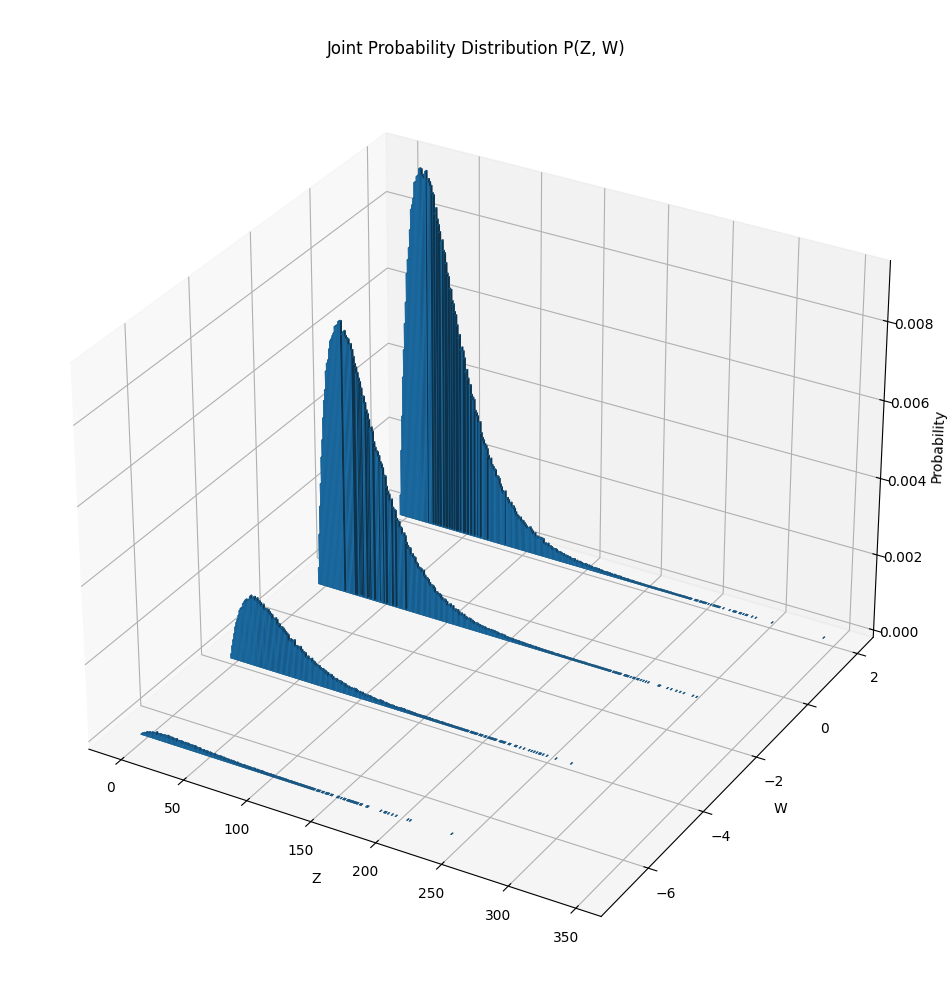
\includegraphics[width=\linewidth]{results/section3/a(2).png}
    \caption{Joint PDF}
  \end{subfigure}
  \begin{subfigure}{\textwidth}
    \inputminted{text}{results/section3/a.txt}
    \caption{Results Output}
  \end{subfigure}
  \caption{Sample Joint Random Variable (Provided on Classroom)}
\end{figure}
\newpage

\begin{figure}[H]
  \centering
  \begin{subfigure}{0.45\textwidth}
    \centering
    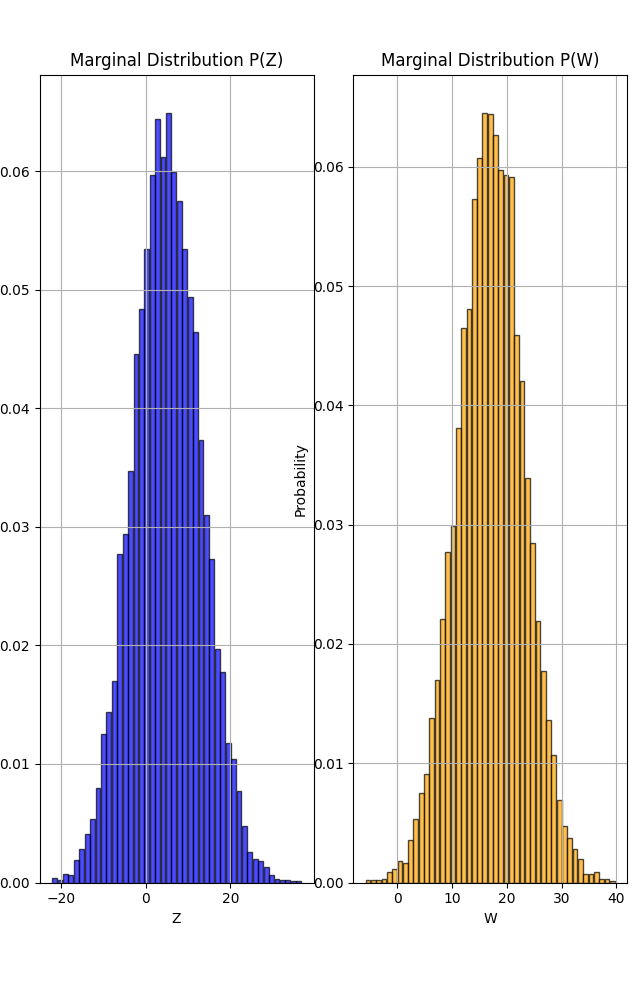
\includegraphics[width=\linewidth]{results/section3/b(1).png}
    \caption{Marginal PDFs}
  \end{subfigure}
  \hfill
  \begin{subfigure}{0.45\textwidth}
    \centering 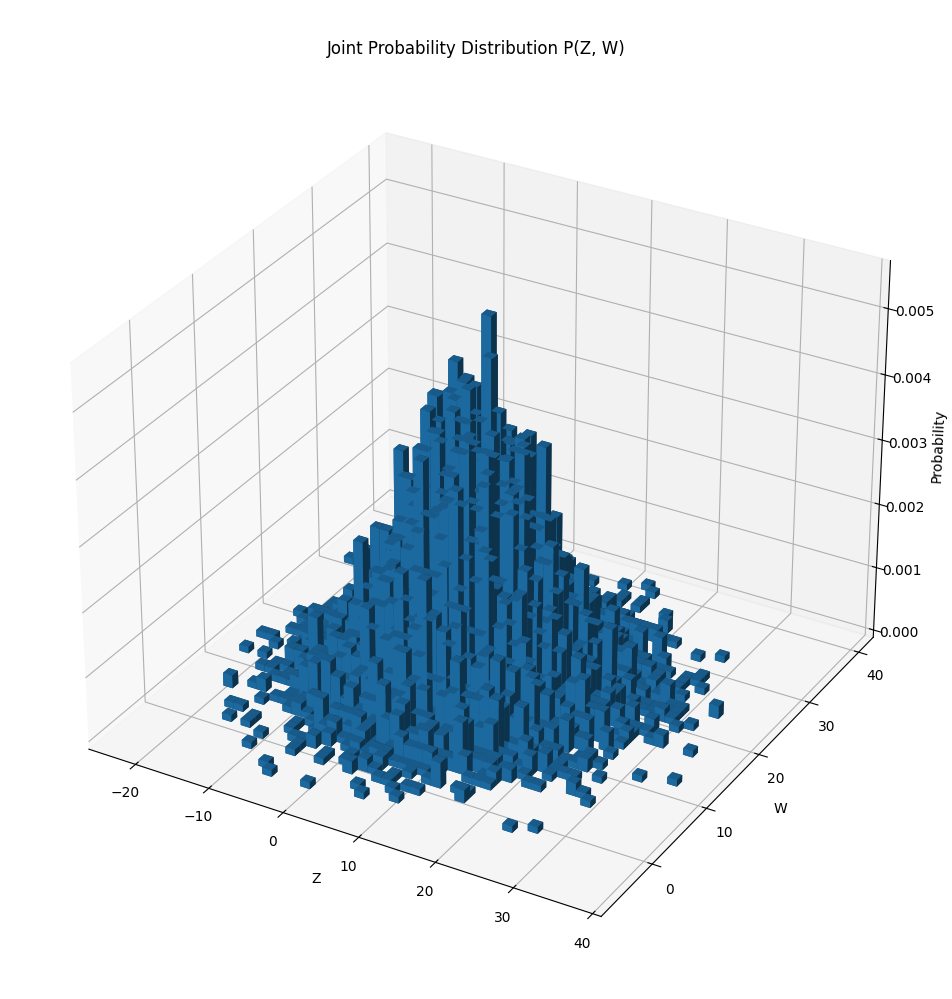
\includegraphics[width=\linewidth]{results/section3/b(2).png}
    \caption{Joint PDF}
  \end{subfigure}
  \begin{subfigure}{\textwidth}
    \inputminted{text}{results/section3/b.txt}
    \caption{Results Output}
  \end{subfigure}
  \caption{$X \sim \mathcal{N}(3, 4)$ and $Y \sim \mathcal{N}(-5,2)$}
\end{figure}
Theoretical Calculations:
Statistical Measurements for Z:
$$E[Z] = 5$$
$$Var(Z) = 64$$

Statistical Measurements for Y:
$$E[Y] = 17$$
$$Var(Y) = 18$$
\newpage

\begin{figure}[H]
  \centering
  \begin{subfigure}{0.45\textwidth}
    \centering
    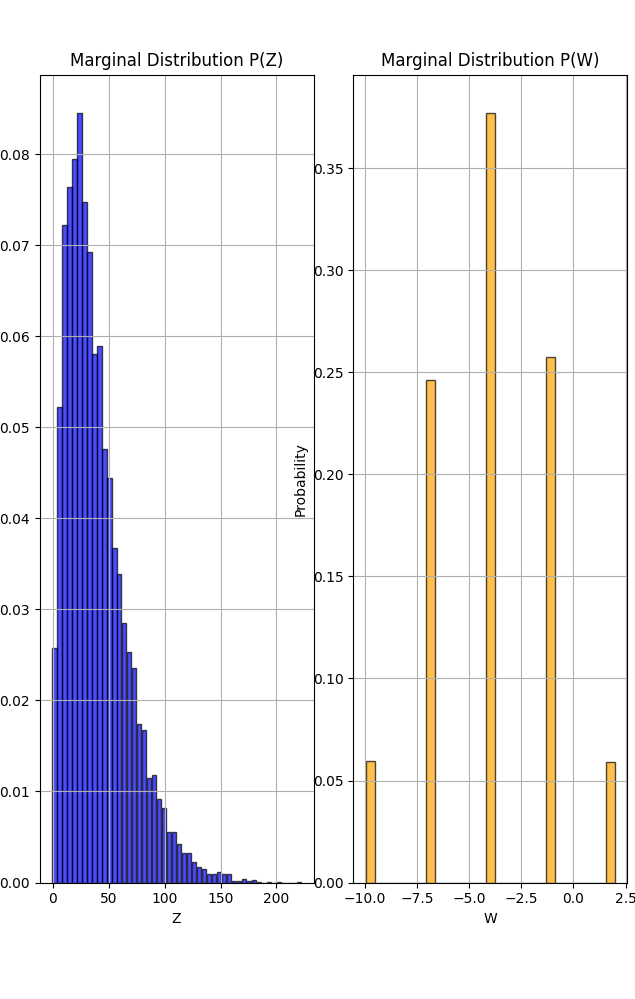
\includegraphics[width=\linewidth]{results/section3/c(1).png}
    \caption{Marginal PDFs}
  \end{subfigure}
  \hfill
  \begin{subfigure}{0.45\textwidth}
    \centering
    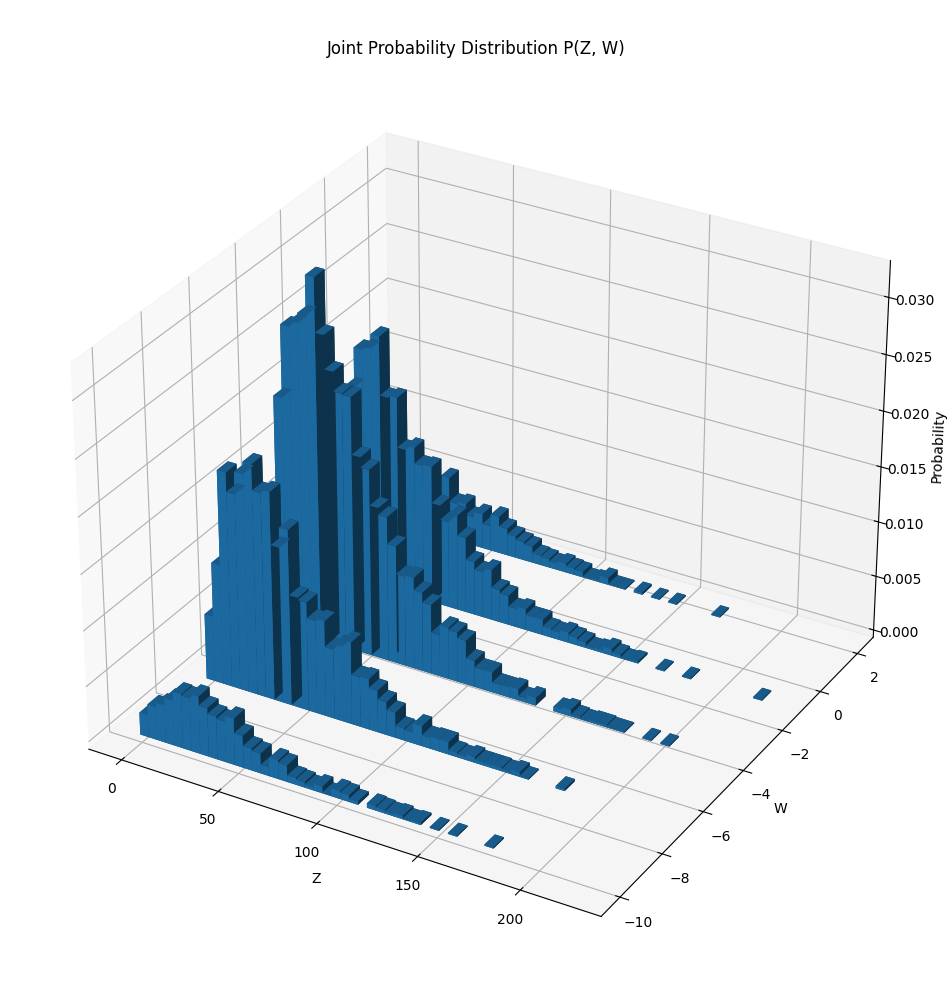
\includegraphics[width=\linewidth]{results/section3/c(2).png}
    \caption{Joint PDF}
  \end{subfigure}
  \begin{subfigure}{\textwidth}
    \centering
    \inputminted{text}{results/section3/c.txt}
    \caption{Results Output}
  \end{subfigure}
  \caption{$X \sim \mathcal{G}amma(2,10)$ and $Y \sim \mathcal{B}in(4,0.5)$}
\end{figure}
Theoretical Calculations:
Statistical Measurements for Z:
$$E[Z] = 39$$
$$Var(Z) = 800$$

Statistical Measurements for Y:
$$E[Y] = -4$$
$$Var(Y) = 9$$
\newpage

\begin{figure}[H]
  \centering
  \begin{subfigure}{0.45\textwidth}
    \centering
    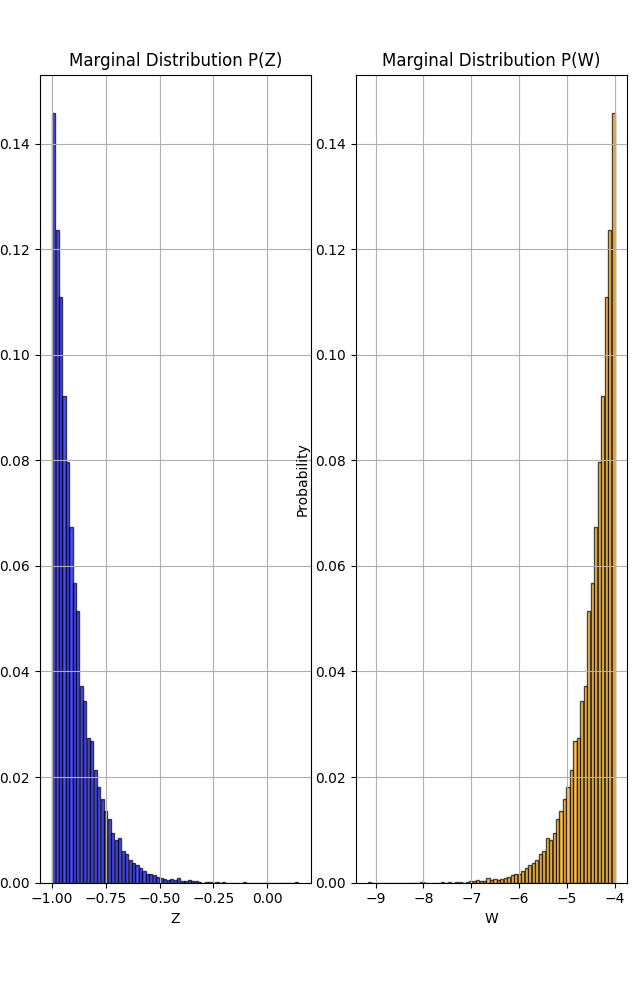
\includegraphics[width=\linewidth]{results/section3/d(1).png}
    \caption{Marginal PDFs}
  \end{subfigure}
  \hfill
  \begin{subfigure}{0.45\textwidth}
    \centering
    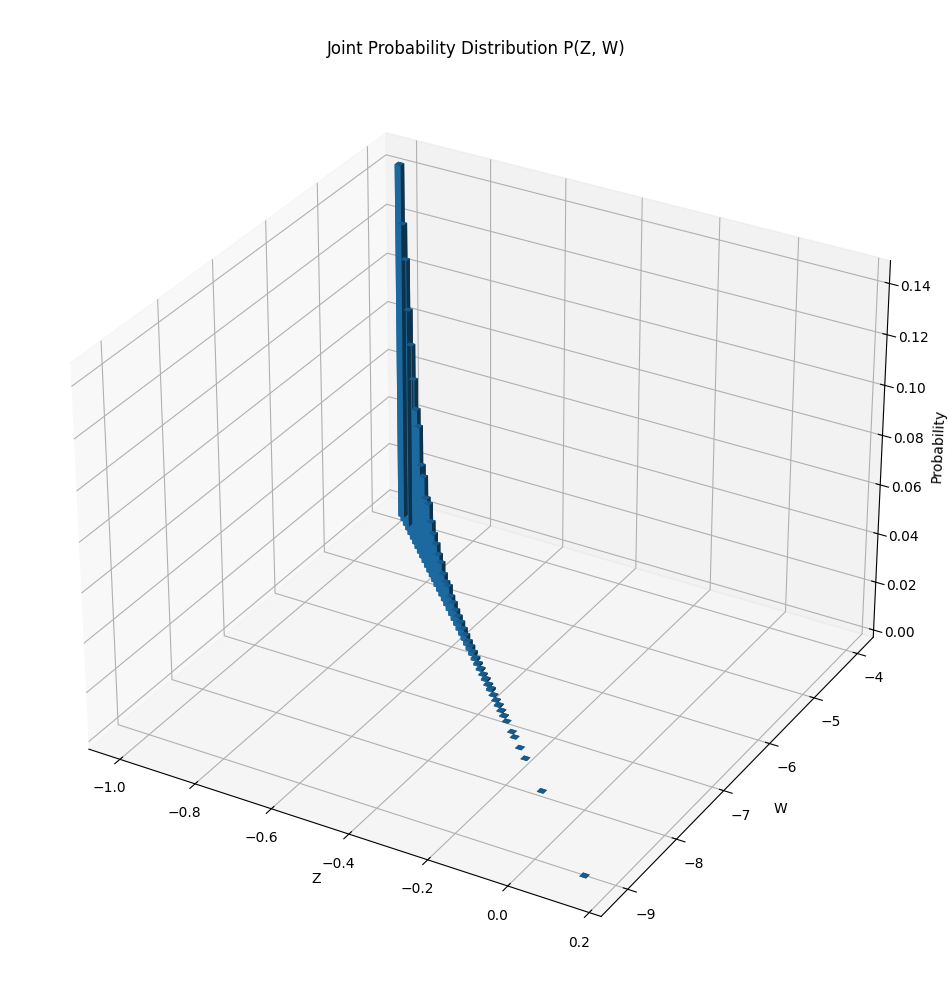
\includegraphics[width=\linewidth]{results/section3/d(2).png}
    \caption{Joint PDF}
  \end{subfigure}
  \begin{subfigure}{\textwidth}
    \centering
    \inputminted{text}{results/section3/d.txt}
    \caption{Results Output}
  \end{subfigure}
  \caption{$X \sim \mathcal{E}xp(0.05)$ and $Y = 3X+2$}
\end{figure}
Theoretical Calculations:
Statistical Measurements for Z:
$$E[Z] = 39$$
$$Var(Z) = 400$$

Statistical Measurements for Y:
$$E[Y] = 17$$
$$Var(Y) = 18$$
\newpage

\begin{figure}[H]
  \centering
  \begin{subfigure}{0.45\textwidth}
    \centering
    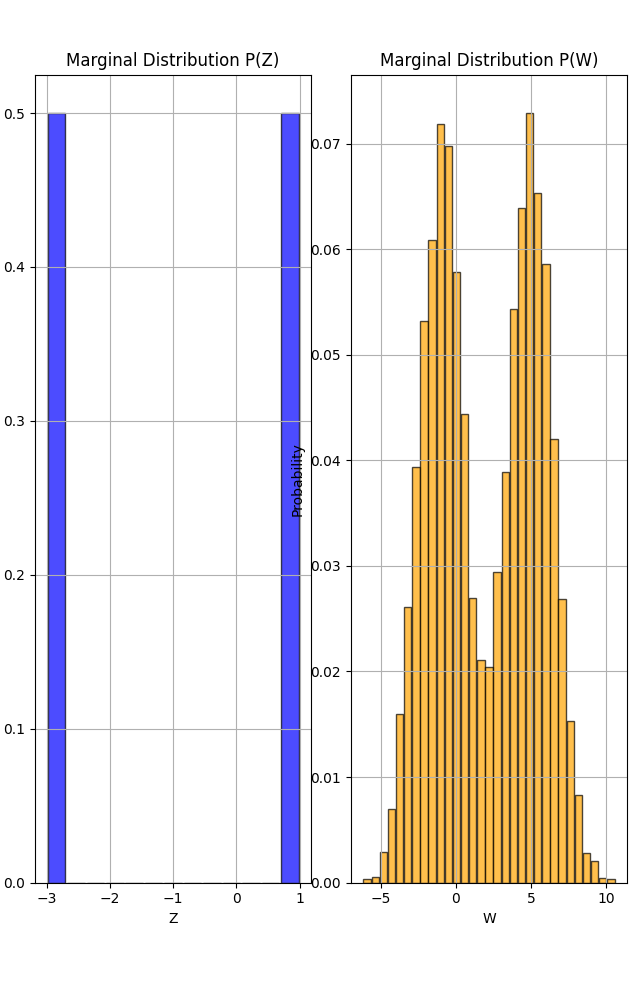
\includegraphics[width=\linewidth]{results/section3/e(1).png}
    \caption{Marginal PDFs}
  \end{subfigure}
  \hfill
  \begin{subfigure}{0.45\textwidth}
    \centering
    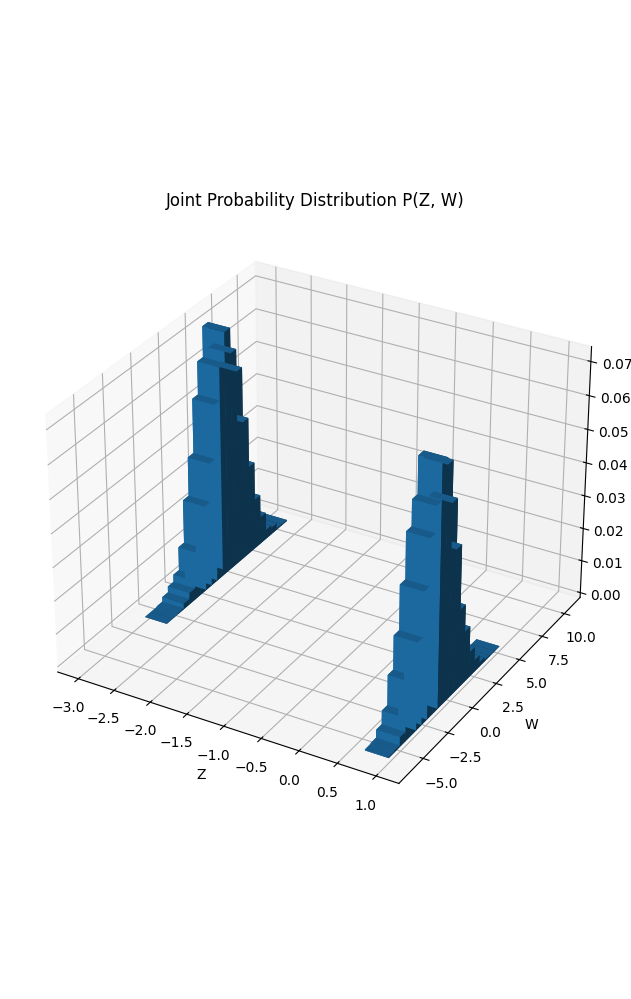
\includegraphics[width=\linewidth]{results/section3/e(2).png}
    \caption{Joint PDF}
  \end{subfigure}
  \begin{subfigure}{\textwidth}
    \centering
    \inputminted{text}{results/section3/e.txt}
    \caption{Results Output}
  \end{subfigure}
  \caption{$X \in \{-1,1\}$ uniform and $Y = X + \mathcal{N}(0, 0.5)$}
\end{figure}
Theoretical Calculations:
Statistical Measurements for Z:
$$E[Z] = -1$$
$$Var(Z) = 4$$

Statistical Measurements for Y:
$$E[Y] = 2$$
$$Var(Y) = 11$$

\newpage

\section{Conclusion}

StatViz.py successfully delivers a versatile and user-friendly tool for analyzing random variables and their statistical properties. This project demonstrates the effective application of Python programming, leveraging libraries such as NumPy, SciPy, Matplotlib, and PyQt6 to create a comprehensive system for statistical analysis and visualization.

The results obtained from the test cases are mostly consistent with theoretical calculations, validating the system's ability to perform accurate statistical analysis. However, discrepancies in certain cases, such as the skewness calculation for the Poisson distribution, highlight areas that may require further investigation and refinement.

StatViz.py is a valuable resource for students, educators, and practitioners interested in exploring and analyzing random variables. Its clear visualizations, along with accurate calculations, help to strengthen understanding of probability theory and statistical concepts. The modular design of the system, along with thorough testing, ensures that the tool is both robust and maintainable, making it suitable for future expansions and enhancements.

Future work may include:

\begin{itemize}
    \item \textbf{Expanding Distribution Support}: Incorporating additional probability distributions for more complex statistical analysis.
    \item \textbf{Improved Discrepancy Handling}: Addressing the discrepancies in the Poisson distribution results through further investigation, as well as refining numeric precision.
    \item \textbf{Interactive Visualization}: Enhancing plots with interactive elements for exploration, zooming, and panning.
     \item \textbf{Statistical Hypothesis Testing}: Integration of common hypothesis tests to provide practical statistical inference capabilities.
    \item \textbf{User Experience Improvements}: Further refinements in GUI design, providing an even more seamless user experience.
\end{itemize}

In summary, StatViz.py provides a strong foundation for statistical analysis and visualization, serving as a practical educational tool and a useful aid in data analysis projects. The tool is not only functional but also provides clear and interactive feedback about the underlying probability distributions. By implementing robust algorithms, utilizing the power of symbolic mathematics, and adopting a clean, user-friendly GUI, StatViz.py empowers users to explore and understand the statistical world around them.

% Bibliography
\nocite{*}
\printbibliography[heading=bibnumbered]

\end{document}
